\documentclass[a4paper,14pt]{extarticle}
\usepackage[utf8]{inputenc}
\usepackage[english,russian]{babel}

\usepackage{amsthm}
\usepackage{graphicx}
\usepackage{caption}
\usepackage{amssymb}
\usepackage{amsmath}
\usepackage{mathrsfs}
\usepackage{euscript}
\usepackage{graphicx}
\usepackage{subfig}
\usepackage{caption}
\usepackage{color}
\usepackage{bm}
\usepackage{tabularx}
\usepackage{adjustbox}
\usepackage{url}

\usepackage[toc,page]{appendix}

\usepackage{comment}
\usepackage{rotating}

\DeclareMathOperator*{\argmax}{arg\,max}
\DeclareMathOperator*{\argmin}{arg\,min}

\newtheorem{theorem}{Теорема}
\newtheorem{lemma}[theorem]{Лемма}
\newtheorem{definition}{Определение}[section]

\numberwithin{equation}{section}

\newcommand*{\No}{No.}

\begin{document}

% Титульный лист
\begin{titlepage}
    	\begin{center}
        		Министерство науки и высшего образования Российской Федерации Федеральное государственное автономное образовательное учреждение высшего образования
       
		«Московский физико-технический институт (национальный исследовательский институт)»

        		Физтех школа прикладной математики и информатики\\
        		Кафедра <<Интеллектуальные системы>>\\
    	\end{center}

    	\vspace{2cm}

    	\begin{center}
       		\Large \bf Выбор структуры моделей глубокого обучения
    	\end{center}
    
    	\begin{center}
		~\\[-28pt]
		Реферат к вступительному испытанию\\
		(Аспирантура)
	\end{center}
	
	\vspace{0.1cm}
	    
    \begin{center}
    	\textbf{Направление подготовки:} 09.06.01 Информатика и вычислительная техника
    \end{center}

   \vspace{0.1cm}

	\begin{flushright}
		\begin{table}[!ht]
			\centering
			\begin{tabular}{l}
				~~~~~~~~~~~~~~~~~~~~~~~~~~~~~~~~~~~~~~~~~~~~~~~~~~ \textbf{Выполнил:}\\
				~~~~~~~~~~~~~~~~~~~~~~~~~~~~~~~~~~~~~~~~~~~~~~~~~~ студент группы М05-904а\\
				~~~~~~~~~~~~~~~~~~~~~~~~~~~~~~~~~~~~~~~~~~~~~~~~~~ Грабовой Андрей Валериевич\\
				~~~~~~~~~~~~~~~~~~~~~~~~~~~~~~~~~~~~~~~~~~~~~~~~~~\\
				~~~~~~~~~~~~~~~~~~~~~~~~~~~~~~~~~~~~~~~~~~~~~~~~~~ \textbf{Научный руководитель:}\\
				~~~~~~~~~~~~~~~~~~~~~~~~~~~~~~~~~~~~~~~~~~~~~~~~~~ Доктор физико-математических наук\\
				~~~~~~~~~~~~~~~~~~~~~~~~~~~~~~~~~~~~~~~~~~~~~~~~~~ Стрижов Вадим Викторович\\
				~~~~~~~~~~~~~~~~~~~~~~~~~~~~~~~~~~~~~~~~~~~~~~~~~~ \\
	    	\end{tabular}
	    \end{table}
	\end{flushright}


	\begin{center}
		Москва 2021
	\end{center}

\end{titlepage}




% Нумерация должна начинаться со второй страницы
\setcounter{page}{2}

% Оглавление
\newpage
\tableofcontents

% Обозначения и сокращения
% \input{./dict.tex}

% Введение
\newpage


\section{Введение}
В силу высокой вычислительной сложности, время оптимизации нейронных сетей может занимать до нескольких дней~\cite{sutskever2014}.
Построение и выбор оптимальной структуры нейронной сети также является вычислительно сложной процедурой, которая значимо влияет на итоговое качество модели. 
При этом алгоритмы оптимизации сходится по большинству параметров сети уже после небольшого числа итераций~\cite{Chunyan2016}.
Своевременное определение начала сходимости параметров позволит существенно снизить вычислительные затраты на обучение моделей с большим числом параметров.
Примерами моделей, с большим число параметров, являются AlexNet~\cite{Krizhevsky2012}, VGGNet~\cite{Simonyan2014}, ResNet~\cite{Kaiming2015}, BERT~\cite{Devlin2018, Vaswani2017}, mT5~\cite{Linting2021}, GPT3\cite{Brown2020} и другие.

Рост числа параметров моделей глубокого обучения влечет снижение интерпретируемости ответов этих моделей.
Первые упоминания о данной проблемы рассмотрены А.\,Г. Ивахненко~\cite{Ivakhnenko1994}.
Проблема с неинтерпретируемыми моделями широко сейчас рассматривается в классе задач по adversarial attack~\cite{Zheng2020}.

Другой проблемой моделей с большим числом параметров является высокие требования к вычислителю в момент предсказания. Использование избыточно сложных моделей с избыточным числом неинформативных параметров является препятствием для использования глубоких сетей на мобильных устройствах в режиме реального времени.
Для снижения числа параметров в литературе рассматривается метод дистилляции модели на основе предсказаний модели учителя~\cite{Hinton2015, Vapnik2015, Lopez2016}.
Модель с большим числом параметров называется учитель. Модель учителя дистиллируется в модель с малым числом параметров, которая называется~ученик.
Основные идеи, которые описывают дистилляцию моделей глубокого обучения предложены в работах Дж.\,Е. Хинтона и В.\,Н. Вапником~\cite{Hinton2015, Vapnik2015, Lopez2016}.
Работы предлагают использовать предсказания модели учителя для повышения качестве модели ученика.
В работе~\cite{Vapnik2015} В.\,Н. Вапником вводится понятие привилегированной информации, которое позволяет использовать дополнительную информацию о данных в момент обучения модели.
Работа~\cite{Lopez2016} объединяет идеи дистилляции~\cite{Hinton2015} с идеями привилегированного обучения~\cite{Vapnik2015}, предложив метод дистилляции модели учителя с большим числом признаков в модель ученика с меньшим числом признаков.
В предложенном методе~\cite{Lopez2016} решается двухэтапная задача. На первом этапе строится модель учителя с расширенным признаковым описанием.
На втором этапе обучается модель ученика в исходном признаковом описании используя дистилляцию~\cite{Hinton2015}.
В работе Дж.\,Е. Хинтона~\cite{Hinton2015} поставлено множество экспериментов по дистилляции моделей глубокого обучения для задачи классификации.
Один из экспериментов проводился на выборке MNIST~\cite{mnist}, который показал, что предложенный дистилляции позволяет построить нейросетевую модель меньшей сложности на основе модели большей сложности.
Второй эксперимент показывал идею по дистилляции ансамбля моделей в одну нейросетевую модель для решения задачи распознания речи. В работе~\cite{Hinton2015} проводится сравнение дистилляции с моделью смеси экспертов.
Дальнейшие работы по дистилляции моделей глубокого обучения рассматривают возможность использования информации о значения параметров модели учителя для оптимизации параметров модели ученика. Работа~\cite{Zehao2017} предлагает метод neuron selectivity transfer, который минимизирует специальную функцию потерь. Данная функция основается на maximum mean discrepancy между выходами слоев модели учителя и модели ученика. В рамках вычислительного эксперимента сравнивалось качество базовой дистилляции с предложенным методов на примере выборок CIFAR~\cite{cifar10} и ImageNet~\cite{imagenet}.

Дистилляция моделей глубокого обучения работает в предположение, что архитектура модели ученика уже известная. Для выборка архитектуры модели ученика предлагается использовать методы прореживания нейросетевых моделей. Существует ряд подходов к построению оптимальной сети. В работах~\cite{maclarin2015, luketina2015} предлагается использовать модель градиентного спуска для оптимизации сети. В~\cite{molchanov2017} используются байесовские методы~\cite{neal1995} оптимизации параметров нейронных сетей. Другим методом поиска оптимальной структуры является прореживание избыточно сложной модели~\cite{cun1990, louizos2017, graves2011}. В работе~\cite{cun1990} предлагается удалять наименее релевантные параметры на основе значений первой и второй производных функции ошибки. В~\cite{grabovoy2019} предложен метод определения релевантности параметров аппроксимирующих моделей при помощи метода Белсли. Релевантность параметров в работе~\cite{grabovoy2019} определяется на основе ковариационной матрицы параметров модели.
Другим примером задания порядка на множестве параметров служит $l_1$-регуляризация~\cite{Tibshirani1996} и регуляризация ElasticNet~\cite{Hastie2005} для линейных моделей.
Порядок, заданный на множестве значений коэффициентов регуляризации, индуцирует порядок на множестве признаковых описаний и указывает на важность признаков.
В случае нейросетей для регуляризации параметров используется метод исключения параметров~\cite{srivastava2014, molchanov2017}.
Данный метод также задает порядок на множестве параметров модели.

Порядок на множестве параметров нейросети можно использовать не только для удаления неимение релевантных параметров, а и для фиксации параметров в процесе оптимизации параметров. Работе~\cite{grabovoy2020} посвящена оптимизации структуры нейронной сети, а также выбору параметров, которые можно зафиксировать после некоторой итерации градиентного метода.

% Основная часть
\newpage

\section{Релевантность параметров параметрических моделей}
Данная работа посвящена прореживанию структуры сети. Предлагается удалять наименее релевантные параметры модели. Под релевантностью~\cite{cun1990} подразумевается то, насколько параметр влияет на функцию ошибки. Малая релевантность указывает на то, что удаление этого параметра не влечет значимого изменения функции ошибки. Метод предлагает построение исходной избыточной сложности нейросети с большим количеством избыточных параметров. Для определения релевантности параметров предлагается оптимизацировать параметры и гиперпараметры в единой процедуре. Для удаления параметров предлагается использовать метод Белсли~\cite{neychev2016}.

\subsection{Постановка задачи к назначению релевантности параметрам модели}

Задана выборка
$$\mathfrak{D} = \{\textbf{x}_i,y_i\},~ i =1,...,N, \eqno(2.1)$$
где $\textbf{x}_i \in \mathbb{R}^{m}$, $y_i \in \{1, \dots, Y\}$, $Y$ --- число классов.
Рассмотрим модель $f(\mathbf{x}, \mathbf{w}): \mathbb{R}^m \times \mathbb{R}^n \to \{1,\dots,Y\}$, где $\textbf{w} \in \mathbb{R}^n$ --- пространство параметров модели,

$$f(\mathbf{x}, \mathbf{w}) = \text{softmax}\bigl( f_1(f_2(...(f_l(\mathbf{x}, \mathbf{w})\bigr), \eqno(2.2)$$
где $f_i(\mathbf{x}, \mathbf{w}) =  \text{tanh}(\mathbf{w}^\mathsf{T}\mathbf{x})$, $l$ --- число слоев нейронной сети, $i \in \{1\dots l\}$.
Параметр $w_j$ модели $f$  называется активным, если $w_j \not = 0$. Множество индексов активных параметров обозначим $\mathcal{A} \subset \mathcal{J} = \{1,...,n\}$.
Задано пространство параметров модели:
$$\mathbb{W_\mathcal{A}} = \{ \textbf{w} \in \mathbb{R}^n~|~w_j\not=0,~j \in \mathcal{A}  \}, \eqno(2.3)$$


Для модели $f$ с множеством индексов активных параметров $\mathcal{A}$ и соответствующего ей вектора параметров $\textbf{w} \in \mathbb{W_\mathcal{A}}$  определим логарифмическую функцию правдоподобия выборки:
$$\mathcal{L}_\mathfrak{D}(\mathfrak{D}, \mathcal{A}, \textbf{w}) = \log p(\mathfrak{D}|\mathcal{A}, \textbf{w}), \eqno(2.4)$$
где $p(\mathfrak{D}|\mathcal{A},\textbf{w})$ --- апостериорная вероятность выборки $\mathfrak{D}$ при заданных $\textbf{w}, \mathcal{A}$.
Оптимальные значения $\textbf{w},\mathcal{A}$ находятся из минимизации $-\mathcal{L}_{\mathcal{A}}(\mathfrak{D},\mathcal{A})$ --- логарифма правдоподобия модели:
$$\mathcal{L}_{\mathcal{A}}(\mathfrak{D},\mathcal{A}) =\log p(\mathfrak{D}|\mathcal{A}) = \log  \int_{{\textbf{w}\in\mathbb{W_\mathcal{J}}}}
p(\mathfrak{D} | \textbf{w}) p(\textbf{w} | \mathcal{A}) d \textbf{w}, \eqno(2.5)$$
где $p(\textbf{w}|\mathcal{A})$ ---  априорная вероятность вектора параметров в пространстве $\mathbb{W_\mathcal{J}}$.

Так как вычисление интеграла (2.5) является вычислительно сложной задачей, рассмотрим вариационный подход~\cite{bishop2006} для решения этой задачи. Пусть задано распределение $q$:
$$q(\textbf{w})\sim \mathcal{N}(\textbf{m}, \textbf{A}^{-1}_\text{ps}), \eqno(2.6)$$
где $\textbf{m}, \textbf{A}^{-1}_\text{ps}$ --- вектор средних и матрица ковариации, аппроксимирующее неизвестное апостериорное распределение $p(\textbf{w}|\mathfrak{D},\mathcal{A})$:
$$p(\textbf{w} | \mathcal{A})\sim \mathcal{N}(\boldsymbol{\mu},\textbf{A}^{-1}_{\text{pr}}), \eqno(2.7)$$
где $\boldsymbol{\mu},\textbf{A}^{-1}_{\text{pr}}$ --- вектор средних и матрица ковариации.

Приблизим интеграл (2.5) методом предложеном в \cite{bishop2006}:
$$\mathcal{L}_{\mathcal{A}}(\mathfrak{D},\mathcal{A}) = \log p(\mathfrak{D}|\mathcal{A}) = $$
$$ =\int_{\textbf{w}\in\mathbb{W_\mathcal{J}}} q(\textbf{w}) \log \frac{p(\mathfrak{D}, \textbf{w}|\mathcal{A})}{q(\textbf{w})}d \textbf{w} - \int_{\textbf{w}\in\mathbb{W_\mathcal{J}}}  q(\textbf{w}) \log \frac{p(\textbf{w}|\mathfrak{D},\mathcal{A})}{q(\textbf{w})}d \textbf{w} \approx $$
$$\approx \int_{\textbf{w}\in\mathbb{W_\mathcal{J}}} q(\textbf{w}) \log \frac{p(\mathfrak{D}, \textbf{w}|\mathcal{A})}{q(\textbf{w})}d \textbf{w} = $$
$$= \int_{\textbf{w}\in\mathbb{W_\mathcal{J}}} q(\textbf{w}) \log \frac{p(\textbf{w}| \mathcal{A})}{q(\textbf{w})}d \textbf{w} + \int_{\textbf{w}\in\mathbb{W_\mathcal{J}}} q(\textbf{w}) \log p(\mathfrak{D}|\mathcal{A}, \textbf{w})d \textbf{w}=$$

$$=\mathcal{L}_\textbf{w}(\mathfrak{D}, \mathcal{A}, \textbf{w})+\mathcal{L}_{E}(\mathfrak{D},\mathcal{A}). \eqno(2.8)$$

Первое слагаемое формулы (2.8) --- это сложность модели. Оно определяется расстоянием Кульбака-Лейблера:
$$\mathcal{L}_\textbf{w}(\mathfrak{D}, \mathcal{A}, \textbf{w}) = -D_{KL}\bigl(q(\textbf{w})||p(\textbf{w}|\mathcal{A})\bigr). \eqno(2.9)$$
Второе слагаемое формулы (2.8) является матожиданием правдоподобия выборки $\mathcal{L}_\mathfrak{D}(\mathfrak{D},\mathcal{A}, \textbf{w})$. В данной работе оно является функцией ошибки:
$$\mathcal{L}_{E}(\mathfrak{D},\mathcal{A}) = \mathsf{E}_{\textbf{w}\sim q}\mathcal{L}_\mathfrak{D}(\textbf{y}, \mathfrak{D}, \mathcal{A}, \textbf{w}). \eqno(2.10)$$

Требуется найти параметры, доcтавляющие минимум суммарному функционалу потерь $\mathcal{L}_\mathcal{A}(\mathfrak{D},\mathcal{A},\textbf{w})$ из (2.8):
$$\hat{\textbf{w}} = \argmin_{\mathcal{A}\subset\mathcal{J},~\textbf{w} \in \mathbb{W_\mathcal{A}}} -\mathcal{L}_\mathcal{A}(\mathfrak{D}, \mathcal{A}, \textbf{w}) = $$
$$=\argmin_{\mathcal{A}\subset\mathcal{J},~\textbf{w} \in \mathbb{W_\mathcal{A}}} D_{KL}\bigl(q(\textbf{w})||p(\textbf{w}|\mathcal{A})\bigr) - \mathcal{L}_\mathfrak{D}(\mathfrak{D}, \mathcal{A}, \textbf{w}). \eqno(2.11)$$

\paragraph{Случайное удаление.}
Метод случайного удаления заключается в том, что случайным образом удаляется некоторый параметр $w_\xi$ из множества активных параметров сети.  Индекс параметра $\xi$ из равномерного распределения  случайная величина, предположительно доставляющая оптимум в (2.11).
$$\xi \sim \mathcal{U}(\mathcal{A}). \eqno(3.1.1)$$

\paragraph{Оптимальное прореживание.}
Метод оптимального прореживания \cite{cun1990} использует вторую производную целевой функции (2.4) по параметрам для определения нерелевантных параметров. Рассмотрим функцию потерь $\mathcal{L}$ (2.4) разложенную в ряд Тейлора в некоторой окрестности вектора параметров $\textbf{w}$:
$$\delta \mathcal{L} = \sum_{j\in \mathcal{A}} g_j\delta w_j + \frac{1}{2}\sum_{i,j\in \mathcal{A}} h_{ij}\delta w_i\delta w_j + O(||\delta\textbf{w}||^3), \eqno(3.2.1)$$
где $\delta w_j $ --- компоненты вектора $\delta\textbf{w}$, $g_j$ --- компоненты вектора градиента $\nabla \mathcal{L}$, а $h_{ij}$ --- компоненты гесcиана $\textbf{H}$:
$$g_j = \frac{\partial \mathcal{L}}{\partial w_j}, \qquad h_{ij} = \frac{\partial^2\mathcal{L}}{\partial w_i \partial w_j}. \eqno(3.2.2)$$

Задача является вычислительно сложной в силу размерности матрицы \textbf{H}. Введем следующее предположение \cite{cun1990}, о том что удаление нескольких параметров приводит к такому же изменению функции потерь $\mathcal{L}$, как и суммарное изменение при индивидуальном удалении:
$$\delta \mathcal{L} = \sum_{j\in \mathcal{A}} \delta \mathcal{L}_j, \eqno(3.2.3)$$
где $\mathcal{A}$ --- множество активных параметров, $\delta\mathcal{L}_j$ --- изменение функции потерь, при удалении одного параметра $\textbf{w}_j$.

В силу данного предположения будем рассматривать только диагональные элементы матрицы \textbf{H}. После введенного предположения, выражение (3.2.1) принимает вид
$$\delta \mathcal{L} = \frac{1}{2} \sum_{j\in \mathcal{A}} h_{jj}\delta w_j^2, \eqno(3.2.4)$$

Получаем следующую задачу оптимизации:

$$\xi = \argmin_{j\in \mathcal{A}} h_{jj}\frac{w_j^2}{2}, \eqno(3.2.5)$$
где $\xi$ --- индекс наименее релевантного, удаляемого параметра, предположительно доставляющая оптимум в (2.11).

\paragraph{Удаление неинформативных параметров с помощью вариационного вывода.}
Для удаления параметров в работе \cite{graves2011} предлагается удалить параметры, которые имеют максимальное отношение плотности $p(\textbf{w}|\mathcal{A})$ априорной вероятности в нуле к плотности вероятности априорной вероятности в математическом ожидании параметра.\\
Для гауссовского распределения с диагональной матрицей ковариации получаем:
$$p_j(\textbf{w}|\mathcal{A})(x) = \frac{1}{\sqrt[]{2\sigma_j^2}}\exp({-\frac{(x-\mu_j)^2}{2\sigma_j^2}}). \eqno(3.3.1)$$
Разделив плотность вероятности в нуле к плотности в математическом ожидание
$$ \frac{p_j(\textbf{w}|\mathcal{A})(0)}{p_j(\textbf{w}|\mathcal{A})(\mu_j)}= \exp({-\frac{\mu_j^2}{2\sigma_j^2}}), \eqno(3.3.2)$$
Получаем следующую задачу оптимизации:
$$\xi = \argmin_{j\in \mathcal{A}} \left|\frac{\mu_j}{\sigma_j}\right|, \eqno(3.3.3)$$
где $\xi$ --- индекс наименее релевантного, удаляемого параметра.

\paragraph{Прореживание сети на основе метода Белсли.}
Предлагается метод основанный на модификации метода Белсли. Пусть $\textbf{w}$ --- вектор параметров доставляющий минимум функционалу потерь $\mathcal{L}$ на  множестве $\mathbb{W_\mathcal{A}}$, а $\textbf{A}_\text{ps}$ соответствующая ему ковариационная матрица.

Выполним сингулярное разложение матрицы
$$\textbf{A}_\text{ps} = \textbf{U}{\bf\Lambda}\textbf{V}^\mathsf{T}. \eqno(4.1)$$
Индекс обусловленности $\eta_{j}$ определим как отношение максимального элемента к $j$-му элементу матрицы ${\bf\Lambda}$. Для нахождения мультиколлиниарных признаков требуется найти индекс $\xi$ вида:
$$\xi = \argmax_{j\in \mathcal{A}}{\eta_j}. \eqno(4.2)$$

\begin{figure}[h!t]\center
\subfloat[Матрица ковариации]{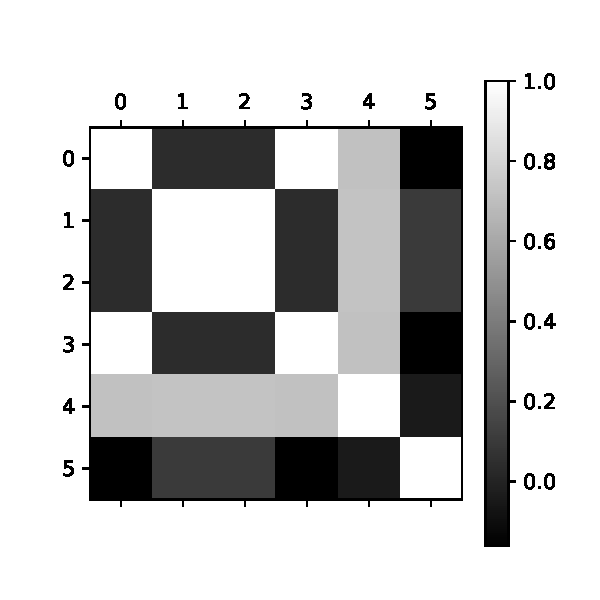
\includegraphics[width=0.5\textwidth]{results/relevant/Cov.pdf}}
\subfloat[Дисперсионные доли]{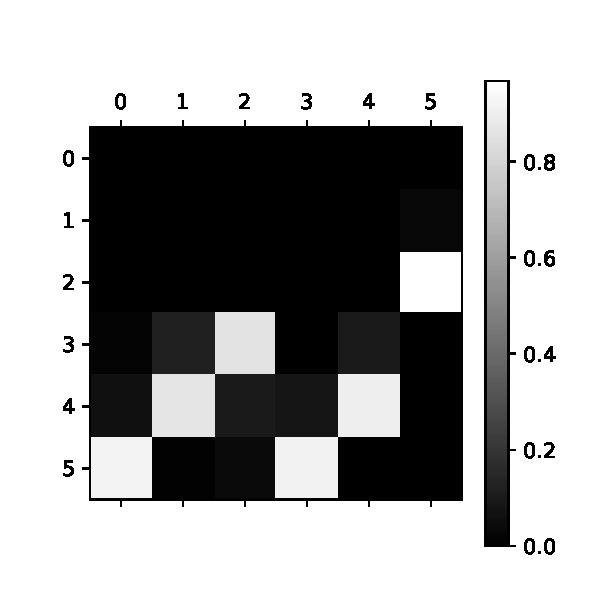
\includegraphics[width=0.5\textwidth]{results/relevant/BelslyImage.pdf}}
\caption{Илюстрация метода Белсли}
\label{CovBel}
\end{figure}

\begin{table}[h]
\begin{center}
\caption{Илюстрация метода Белсли}
\begin{tabular}{|c|cccccc|}
\hline
$\eta$ & $q_1$& $q_2$& $q_3$& $q_4$& $q_5$& $q_6$\\
\hline
$1.0$ &  $2\cdot 10^{-17}$ &  $4\cdot 10^{-17}$ &  $1\cdot 10^{-16}$ &  $2\cdot 10^{-17}$ &  $6\cdot 10^{-17}$&  $3\cdot 10^{-4}$ \\
\hline
$1.5$ &  $5\cdot 10^{-17}$ &  $9\cdot 10^{-17}$ &  $2\cdot 10^{-16}$ &  $5\cdot 10^{-17}$ &  $3\cdot 10^{-20}$ &  $3\cdot 10^{-2}$ \\
\hline
$3.3$ &  $9\cdot 10^{-18}$ &  $1\cdot 10^{-17}$ &  $2\cdot 10^{-17}$ &  $9\cdot 10^{-18}$ &  $2\cdot 10^{-19}$ &  $9\cdot 10^{-1}$ \\
\hline
$2\cdot 10^{15}$ &  $1\cdot 10^{-2}$ &  $1\cdot 10^{-1}$ &  $8\cdot 10^{-1}$ &  $2\cdot 10^{-3}$ &  $9\cdot 10^{-2}$ &  $1\cdot 10^{17}$ \\ 
\hline
$8\cdot 10^{15}$ &  $6\cdot 10^{-2}$ &  $8\cdot 10^{-1}$ &  $9\cdot 10^{-2}$ &  $8\cdot 10^{-2}$ &  $9\cdot 10^{-1}$ & $ 2\cdot 10^{17} $\\
\hline
$1\cdot 10^{16}$ &  $\bf9\cdot 10^{-1}$ &  $1\cdot 10^{-2}$& $ 4\cdot 10^{-2}$&  $\bf9\cdot 10^{-1}$ &  $1\cdot 10^{-3}$ & $ 5\cdot 10^{-21}$ \\
\hline
\end{tabular}
\label{CovBelTable}
\end{center}
\end{table}

Дисперсионный долевой коэффициент $q_{ij}$ определим как вклад $j$-го признака в дисперсию $i$-го элемента вектора параметра $\textbf{w}$:

$$q_{ij} = \frac{u^2_{ij}/\lambda_{jj}}{\sum^n_{j=1}{u^2_{ij}/\lambda_{jj}}}. \eqno(4.3)$$

Большие значение дисперсионных долей указывают на наличие зависимости между параметрами. Находим долевые коэффициенты, которые вносят максимальный вклад в дисперсию параметра $w_\xi$:

$$\zeta = \argmax_{j\in \mathcal{A}}{q_{\xi j}}. \eqno(4.4)$$
Параметр с индексом $\zeta$ определим как наименее релевантный параметр нейросети. 
%Для удаления нескольких зависимых параметров за раз, предлагается удалить параметры с номерами $p \in \mathcal{A}: q_{\xi i} > \lambda  \in  \mathbb{R}_+$.

Проиллюстрируем принцип работы метода Белсли на примере. Рассмотрим данные порожденные следующим образом: 
$$\textbf{w} = \begin{bmatrix}
\text{sin}(x)\\
\text{cos}(x)\\
\text{2+cos}(x)\\
\text{2+sin}(x)\\
\text{cos}(x) + \text{sin}(x)\\
x
\end{bmatrix}$$
с матрицей ковариации на рис.~\ref{CovBel}.a, где $x \in [0.0, 0.02, ..., 20.0]$.


В табл.~\ref{CovBelTable} приведены индексы обусловленности и соответствующие им дисперсионные доли, которые также изображены на рис.~\ref{CovBel}.b. Согласно этим данным, максимальный индекс обусловленности $\eta_6 = 1.2\cdot 10^{16}$. Ему соответствуют максимальные дисперсионные доли признаков с индексами 1 и 4, которые, как видно из построения выборки, являются линейно зависимые.

\subsection{Анализ разных подходов к определению релевантности}
Для анализа свойств предложенного алгоритма и сравнения его с существующими был проведен вычислительный эксперимент в котором параметры нейросети удалялись методами,  которые были описаны в разделах 3.1---3.3 и методом Белсли.

В качестве данных использовались три выборки. Выборки Wine \cite{Wine} и Boston Housing \cite{Boston}  --- это реальные данные. Синтетические данные сгенерированы таким образом чтобы параметры сети были мультиколинеарными. Генерация данных состояла из двух этапов. 
На первом этапе генерировался вектор параметров $\mathbf{w}_{\text{synthetic}}$:
$$\mathbf{w}_{\text{synthetic}}  \sim \mathcal{N}(\textbf{m}_{\text{synthetic}}, \textbf{A}_{\text{synthetic}}), \eqno(5.1)$$ 
где 
$\textbf{m}_{\text{synthetic}} = \begin{bmatrix}
1.0\\
0.0025\\
\cdots\\
0.0025
\end{bmatrix}$,
$\textbf{A}_{\text{synthetic}} = \begin{bmatrix}
1.0& 10^{-3}& \cdots& 10^{-3}& 10^{-3}\\
10^{-3}& 1.0& \cdots& 0.95& 0.95\\
\cdots&\cdots&\cdots&\cdots&\cdots\\
10^{-3}& 0.95& \cdots& 0.95& 1.0
\end{bmatrix}$.

На втором этапе генерировалась выборка $\mathfrak{D}_{\text{synthetic}}$:
$$\mathfrak{D}_{\text{synthetic}} = \{(\textbf{x}_i,y_i)| \textbf{x}_i \sim  \mathcal{N}(\textbf{1}, \textbf{I}), y_i = x_{i0}, i = 1 \cdots 10000\}. \eqno(5.2)$$
В приведенном выше векторе параметров $\mathbf{w}_{\text{synthetic}}$ для выборки $\mathfrak{D}_{\text{synthetic}}$, наиболее релевантным является первый параметр, а все остальные параметры являются нерелевантными. Матрица ковариации была выбрана таким образом, чтобы все нерелевантные параметры были зависимы и метод Белсли был максимально эффективен.



\begin{table}[h]

\begin{center}
\caption{Описание выборок}
\begin{tabular}{|c|c|c|c|}
\hline
	Выборка &Тип задачи& Размер выборки& Число признаков\\
	\hline
	
	\multicolumn{1}{|l|}{Wine}
	&
	\multicolumn{1}{|l|}{класификация}
	 & 178 & 13\\
	\hline
	
	\multicolumn{1}{|l|}{Boston Housing}
	&
	\multicolumn{1}{|l|}{регресия}
	& 506 & 13\\
	\hline
	
	\multicolumn{1}{|l|}{Synthetic data}
	&
	\multicolumn{1}{|l|}{регресия}
	& 10000 & 100\\
\hline

\end{tabular}
\end{center}
\end{table}



Для алгоритмов тренировочная и тестовая выборки составили $80\%$ и $20\%$ соответсвенно. Критерием качества прореживания служит процент параметров нейросети, удаление которого не влечет значимой потери качества прогноза. Также критерием качества служит устойчивость нейросети к зашумленности данных. 

Качеством прогноза $R_{\text{cl}}$ модели для задачи классификации является точность прогноза модели:
$$R_{\text{cl}} = \frac{\sum_{(\textbf{x},y)\in \mathfrak{D}} [f(\textbf{x}, \textbf{w}) = y]}{\left|\mathfrak{D}\right|}, \eqno(5.3)$$

Качеством прогноза $R_{\text{rg}} $ модели для задачи регрессии является среднеквадратическое отклонение результата модели от точного:

$$R_{\text{rg}} = \frac{\sum_{(\textbf{x},y)\in \mathfrak{D}} \left(f(\textbf{x}, \textbf{w}) - y\right)^2}{\left|\mathfrak{D}\right|}, \eqno(5.4)$$

\paragraph{Wine.} Рассмотрим нейроную сеть с 13 нейронами на входе, 13 нейронами в скрытом слое и 3 нейронами на выходе.

\begin{figure}[h!t]\center
\includegraphics[width=0.8\textwidth]{results/relevant/WIne/All.pdf}\\
\caption{Качество прогноза при удаление параметров на выборке Wine}
\label{WineAll}
\end{figure}

\begin{figure}[h!t]\center
\subfloat[Произвольное удаление параметров]{\includegraphics[width=0.5\textwidth]{results/relevant/WIne/RandomNoise3D.pdf}}
\subfloat[Оптимальное прореживание]{\includegraphics[width=0.5\textwidth]{results/relevant/WIne/OBDNoise3D.pdf}}\\
\subfloat[Вариационный метод]{\includegraphics[width=0.5\textwidth]{results/relevant/WIne/VariationalNoise3D.pdf}}
\caption{Влияние шума в начальных данных на шум выхода нейросети на выборке Wine}
\label{WineNoise}
\end{figure}

На рис.~\ref{WineAll} показано как меняется точность прогноза $R_{\text{cl}}$ при удалении параметров указанными методами. Из графика видно, что метод оптимального прореживания, вариационный метод и метод Белсли позволяют удалить $\approx80\%$ параметров и качество всех этих методов падает при удалении $\approx90\%$ параметров нейросети. 

На рис.~\ref{WineNoise} показаны поверхности изменения уровня шума ответов нейросети при изменении процента удаленных параметров и уровня шума входных данных для разных методов прореживания. На графиках показано, что при удалении параметров нейросети методом Белсли шум меньше, чем при удалении параметров другими методами, на это указывает то что поверхность которая соответствует методу Белсли ниже других поверхностей.

\paragraph{Boston Housing.} Рассмотрим нейроную сеть с 13 нейронами на входе, 39 нейронами в скрытом слое и одним нейроном на выходе.

\begin{figure}[h!t]\center
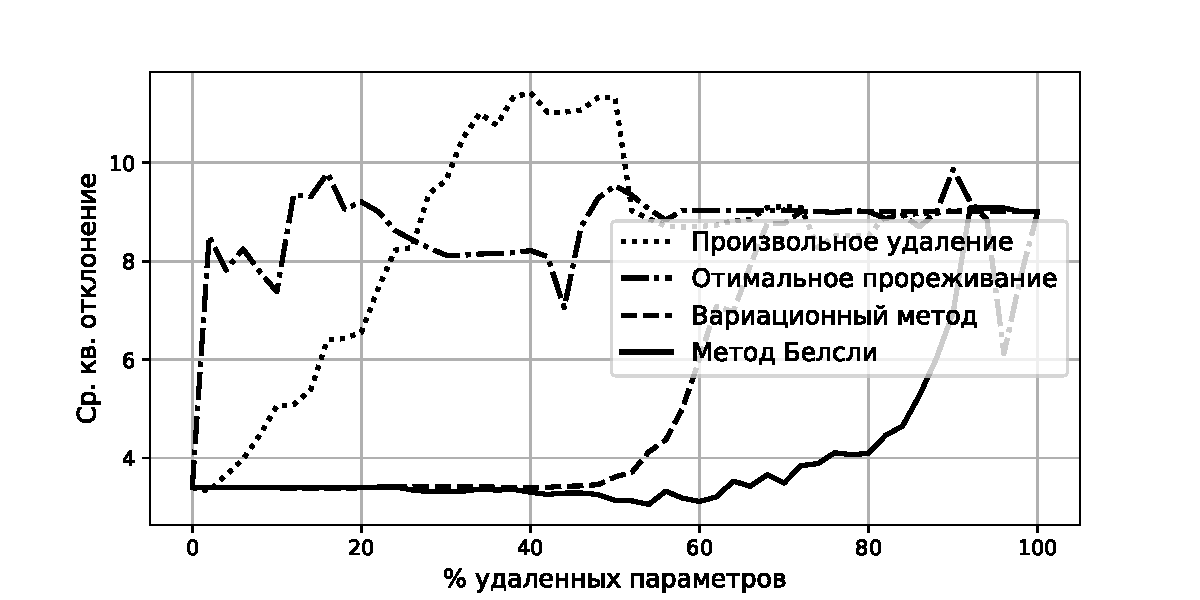
\includegraphics[width=0.8\textwidth]{results/relevant/Boston/All.pdf}\\
\caption{Качество прогноза при удаление параметров на выборке Boston}
\label{BostonAll}
\end{figure}

\begin{figure}[h!t]\center
\subfloat[Произвольное удаление параметров]{\includegraphics[width=0.5\textwidth]{results/relevant/Boston/RandomNoise3D.pdf}}
\subfloat[Оптимальное прореживание]{\includegraphics[width=0.5\textwidth]{results/relevant/Boston/OBDNoise3D.pdf}}\\
\subfloat[Вариационный метод]{\includegraphics[width=0.5\textwidth]{results/relevant/Boston/VariationalNoise3D.pdf}}
\caption{Влияние шума в начальных данных на шум выхода нейросети на выборке Boston}
\label{BostonNoise}
\end{figure}

На рис.~\ref{BostonAll} показано как меняется среднеквадратическое отклонение прогноза $\mathsf{R}_{\text{rg}}$ от точного ответа  при удалении параметров указанными методами. График показывает, что метод Белсли является более эффективным, чем другие методы, так-как позволяет удалить больше параметров нейросети без потери качества.

На рис.~\ref{BostonNoise} показаны поверхности изменения уровня шума ответов нейросети при изменении процента удаленных параметров и уровня шума входных данных для разных методов прореживания. График показывает, что уровень шума всех методов одинаковый, так-как поверхности всех методов находятся на одном уровне.


\paragraph{Синтетические данные.} Рассмотрим нейроную сеть с 100 нейронами на входе и одним нейроном на выходе.

\begin{figure}[h!t]\center
\includegraphics[width=0.8\textwidth]{results/relevant/Data1/All.pdf}\\
\caption{Качество прогноза при удаление параметров на синтетической выборке}
\label{Data1All}
\end{figure}

\begin{figure}[h!t]\center
\subfloat[Произвольное удаление параметров]{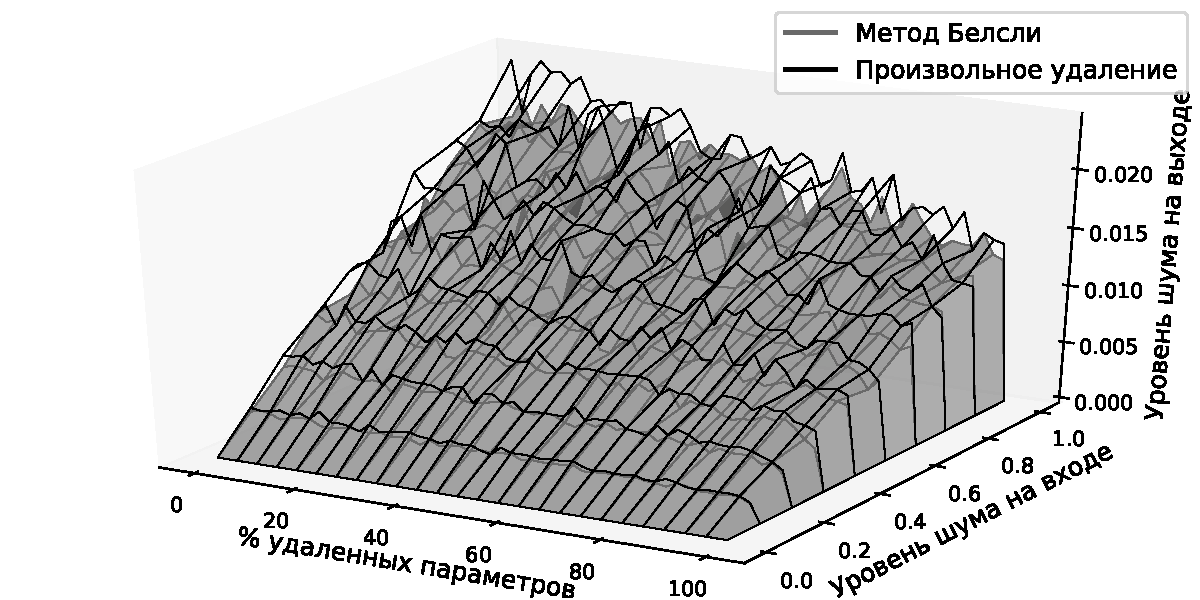
\includegraphics[width=0.5\textwidth]{results/relevant/Data1/RandomNoise3D.pdf}}
\subfloat[Оптимальное прореживание]{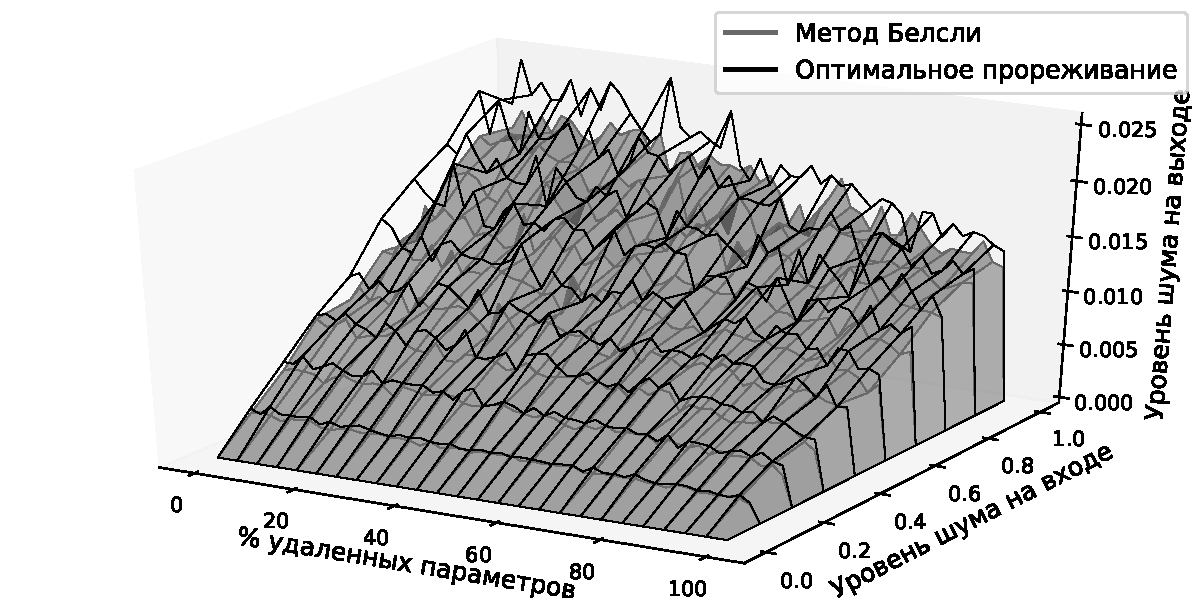
\includegraphics[width=0.5\textwidth]{results/relevant/Data1/OBDNoise3D.pdf}}\\
\subfloat[Вариационный метод]{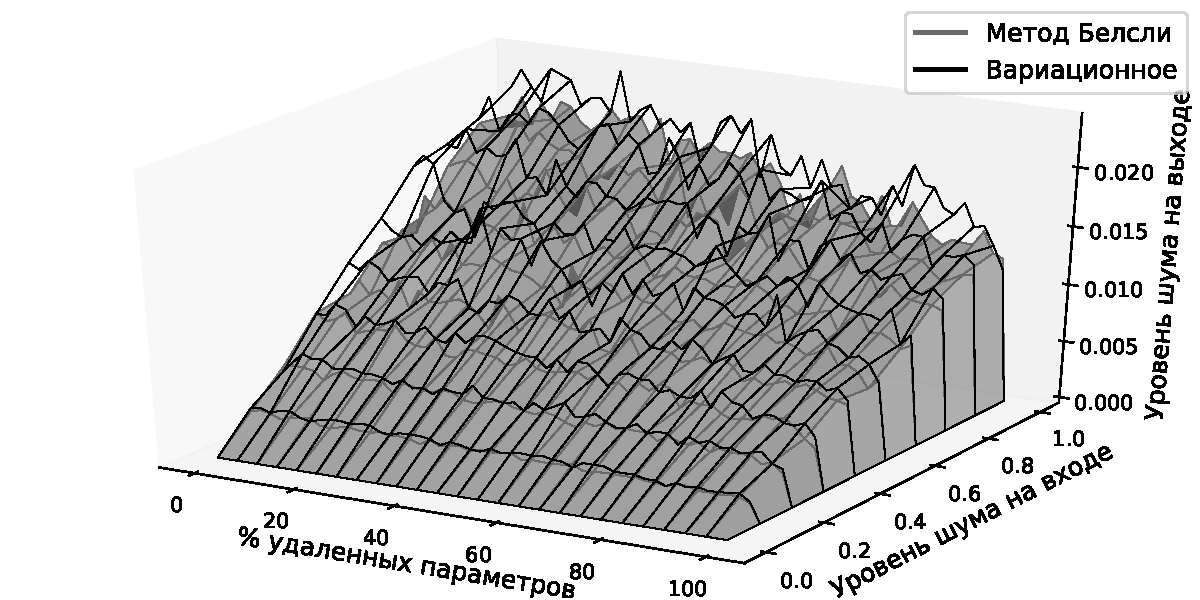
\includegraphics[width=0.5\textwidth]{results/relevant/Data1/VariationalNoise3D.pdf}}
\caption{Влияние шума в начальных данных на шум выхода нейросети на синтетической выборке}
\label{Data1Noise}
\end{figure}

На рис.~\ref{Data1All} показано как меняется среднеквадратическое отклонение прогноза от $\mathsf{R}_{\text{rg}}$ точного ответа при удалении параметров указанными методами. График показывает, что удаление параметров методом Белсли являеться более эффективным чем другие методы прореживания, так-как качество прогноза нейросети улучшается при удалении шумовых параметров.

На рис.~\ref{Data1Noise} показаны поверхности изменения уровня шума ответов нейросети при изменении процента удаленных параметров и уровня шума входных данных для разных методов прореживания. На графиках показано, что при удалении параметров нейросети методом Белсли шум меньше, чем при удалении параметров другими методами, так-как поверхность которая соответствует методу Белсли ниже других поверхностей.

\newpage

\section{Введение отношения порядка на множестве параметров аппроксимирующих моделей}
В данной работе предлагается метод введения отношения порядка на множестве параметров сложных параметрических моделей, таких как нейросеть. Рассматривается порядок, заданный при помощи ковариационной матрицы градиентов функции ошибки по параметрам модели \cite{Mandt2017}. В работе \cite{Chunyan2016} предложен итерационный метод для поиска ковариационной матрицы градиентов. Данный итерационный метод интегрируется в градиентный метод оптимизации Adam \cite{kingma2014}.

Множество параметров упорядочивается по возрастанию дисперсии: от параметра с минимальной дисперсией до параметра с максимальной дисперсией градиента функции ошибки по соответствующему параметру модели. Предполагается, что малая дисперсия градиента указывает на то, что соответствующий параметр можно зафиксировать.

Для задания порядка на множестве параметров при помощи ковариационной матрицы вводится предположение о том, что фиксация параметров происходит в момент, когда все параметры модели находятся в некоторой окрестности локального минимума функции ошибки. Данное условие накладывается для корректного использования итерационного метода поиска ковариационной матрицы градиентов.

Заданный порядок на множестве параметров модели используется для фиксации тех параметров модели, которые оказываются предстоящими с точки зрения заданного порядка. Сначала фиксируются те параметры, которые имеют минимальную дисперсию градиента в окрестности локального минимума функции ошибки.

Для анализа свойств предложенного метода задания порядка на множестве параметров проводился вычислительный эксперимент. В качестве моделей рассматривались модели различной структурной сложности: линейные модели, нейросетевые модели. Предложенный метод задания порядка сравнивается с методом, в котором порядок задан произвольным образом.
\subsection{Задача упорядочивания параметров аппроксимирующих моделей}
Задана выборка:
\[
\label{eq:st:1}
\begin{aligned}
\mathfrak{D} = \bigr\{\bigr(\textbf{x}_i, y_i\bigr)\bigr\}_{i=1}^{m}, \quad \textbf{x}_{i} \in \mathbb{X} = \mathbb{R}^{n}, \quad y_i \in \mathbb{Y},
\end{aligned}
\]
где $n$ --- размерность признакового пространства, $m$ --- число объектов в выборке. Пространство ответов $\mathbb{Y} = \mathbb{R}$ в случае задачи регрессии и  $\mathbb{Y} = \{1,\cdots, K\}$ в случае задачи классификации, где $K$ --- число классов.

Задано семейство моделей параметрических функций с наперед заданной структурой:
\[
\label{eq:st:2}
\begin{aligned}
\mathfrak{F} &= \bigr\{f\bigr(\textbf{w}\bigr):\mathbb{X} \to \mathbb{Y} | \textbf{w} \in \mathbb{R}^{p}\bigr\}, \\ 
\mathbf{h}\bigr(\textbf{w}, \textbf{x}\bigr) &= \textbf{W}_1\bm{\sigma}\bigr(\textbf{W}_2\bm{\sigma}\bigr(\cdots\bm{\sigma}\bigr(\textbf{W}_r\textbf{x}\bigr)\cdots\bigr)\bigr),\\
f_{\text{\text{cl}}}\bigr(\textbf{w}, \textbf{x}\bigr) &= \arg \max_{j \in \bigr\{1,\cdots, K\bigr\}} \text{softmax}\bigr(\mathbf{h}\bigr(\textbf{w}, \textbf{x}\bigr)\bigr)_{j}, \\ 
f_{\text{reg}}\bigr(\textbf{w}, \textbf{x}\bigr) & = \mathbf{h}\bigr(\textbf{w}, \textbf{x}\bigr), 
\end{aligned}
\]
где $p$ --- размерность пространства параметров, $r$ --- число слоев нейросети, $\textbf{w} = \text{vec}[\textbf{W}_1, \textbf{W}_2, \cdots, \textbf{W}_r]$, а $\bm{\sigma}$ --- функция активации. В случае задачи регрессии структура модели имеет вид $f_{\text{\text{reg}}}$, а в случае классификации имеет вид $f_{\text{\text{cl}}}$.
%В качестве $\tau$ рассматривается $\tau\bigr(\textbf{x}\bigr) = \textbf{x}$ в случае задачи регрессии, в случае задачи многоклассовой классификации $\bm{\sigma}\bigr(\textbf{x}\bigr) = \text{softmax}\bigr(\textbf{x}\bigr)$.
Задана функция потерь:
\[
\label{eq:st:3}
\begin{aligned}
\mathcal{L}\bigr(\textbf{w}, \mathfrak{D}\bigr) &= \frac{1}{m}\sum_{i=1}^{m}l\bigr(\textbf{x}_{i}, y_i, \textbf{w}\bigr),\\
l_{\text{\text{reg}}}\bigr(\textbf{x}, y, \textbf{w}\bigr) &= \bigr(y - f\bigr(\textbf{w}, \textbf{x}\bigr)\bigr)^{2},\\
l_{\text{\text{cl}}}\bigr(\textbf{x}, y, \textbf{w}\bigr) &= -\sum_{j=1}^{K}\bigr([y = j]\ln\text{softmax}_j\bigr(\mathbf{h}\bigr(\textbf{w}, \textbf{x}\bigr)\bigr)\bigr),
\end{aligned}
\]
где $l_{\text{\text{reg}}}$ --- это функция ошибки на одном элементе для задачи регрессии, $l_{\text{\text{cl}}}$ --- для задачи классификации.
Оптимальный вектор параметров $\hat{\textbf{w}}$ получим минимизацией функции потерь:
\[
\label{eq:st:0:1}
\begin{aligned}
\hat{\textbf{w}} = \arg \min_{\textbf{w}\in\mathbb{R}^{p}} \mathcal{L}\bigr(\textbf{w}, \mathfrak{D}\bigr).
\end{aligned}
\]

Для поиска оптимальных параметров модели используется градиентный метод оптимизации:
\[
\label{eq:st:4}
\begin{aligned}
\textbf{w}_{t} = \textbf{w}_{t-1} + \Delta\textbf{w}\bigr(\textbf{g}_{S,t}, \textbf{w}_{t-1}, \textbf{w}_{t-2}, \cdots\bigr), \quad \textbf{g}_{S,t}=\frac{\partial \mathcal{L}\bigr(\textbf{w}_{t}, \textbf{X}_{S}, \textbf{Y}_{S}\bigr)}{\partial \textbf{w}},
\end{aligned}
\]
где $t$ --- номер итерации, $\textbf{g}_{S,t}$ --- значение градиента на подвыборке размера $S$, $\Delta\textbf{w}$ --- приращение вектора параметров.
 
 
Порядок на множестве параметров модели задается при помощи ковариационной матрицы $\textbf{C}$ градиентов функции ошибки $\mathcal{L}$ по параметрам модели $\textbf{w}$. Для вычисления ковариационной матрицы $\textbf{C}$ используется итерационная формула \cite{Chunyan2016}, которая вычисляется на каждой итерации \eqref{eq:st:4} градиентного метода оптимизации параметров:
\[
\label{eq:st:5}
\begin{aligned}
\textbf{C}_t = \bigr(1-\kappa_t\bigr)\textbf{C}_{t-1}+\kappa_t\bigr(\textbf{g}_{1,t}-\textbf{g}_{S,t}\bigr)\bigr(\textbf{g}_{1,t}-\textbf{g}_{S,t}\bigr)^{\mathsf{T}},
\end{aligned}
\]
 где $t$ --- номер итерации, $\textbf{g}_{S,t}$ --- значение градиента на подвыборке размера $S$, $\textbf{g}_{1,t}$ --- значение градиента на первом элементе подвыборки, $\kappa_t=\frac{1}{t}$ --- параметр сглаживания, $\textbf{C}_0$ инициализируются из равномерного распределения.
 
Пусть известно $t_0$ --- число итераций, после которого все параметры находятся в некоторой локальной окрестности минимума, тогда, как показано в работе \cite{Chunyan2016}, матрица $\textbf{C}_{t_0}$ аппроксимирует истинную ковариационную матрицу $\textbf{C}$. Ковариационная матрица $\textbf{C}_{t_0}$ используется для упорядочения параметров модели $\textbf{w}_{t_0}$. 
 
Пусть $\mathcal{I}$ ---  упорядоченный вектор индексов $[1, 2, \cdots, p]$. Обозначим $\mathcal{I}_{\textbf{w}_{t_0}}$ вектор индексов, порядок которого задан при помощи ковариационной матрицы $\textbf{C}_{t_0}$. 
 
Например, если ковариационная матрица $\textbf{C}_{t_0}$  имеет вид
 $$
\begin{bmatrix}
0{,}3& 0 & 0\\
0& 0{,}2 & 0\\
0& 0 & 0{,}25\\
\end{bmatrix},
 $$
 то вектор индексов $\mathcal{I}_{\textbf{w}_{t_0}} = [3,1,2]$.
 

\subsection{Фиксация параметров модели в процессе обучения}
Для фиксации параметров $\textbf{w}_{t_0}$ при помощи вектора индексов $\mathcal{I}_{\textbf{w}_{t_0}}$ используется бинарный вектор $\bm{\alpha}\bigr(k\bigr)$:
\[
\label{eq:st:6}
\begin{aligned}
\alpha_i\bigr(k\bigr) = \begin{cases}
   1, &\text{если }\mathcal{I}_{\textbf{w}_{t_0}}[j] \leq k;\\
   0 &\text{иначе},
 \end{cases}
\end{aligned}
\]
 где $k$ --- число фиксирующих параметров.
 
 Учитывая \eqref{eq:st:6}, уравнение \eqref{eq:st:4} приводится к виду
 \[
\label{eq:st:7}
\begin{aligned}
\textbf{w}_{t} = \textbf{w}_{t-1} + \bm{\alpha}\bigr(k\bigr)\cdot\Delta\textbf{w}\bigr(\textbf{g}_{S,t}, \textbf{w}_{t-1}, \textbf{w}_{t-2}, \cdots\bigr),
\end{aligned}
\]
где $t$ --- номер итерации, $\textbf{g}_{S,t}$ --- значение градиента на подвыборке размера $S$, $\Delta\textbf{w}$ --- приращение вектора параметров. После умножения на бинарный вектор $\bm\alpha$ часть параметров не оптимизируется, что приводит к фиксации параметров.

\subsection{Вычислительный эксперимент по упорядочиванию параметров}

\begin{table}[h!t]
\begin{center}
\caption{Описание выборок, используемых в эксперименте}
\label{tb:ex:1}
\begin{tabular}{|c|c|c|c|c|c|}
\hline
	Выборка, $\mathfrak{D}$& Тип & Число& Модель& Число \\
	&& признаков, $n$&&параметров, $p$\\
	\hline
	\multicolumn{1}{|l|}{Boston Housing}&
	Регрессия& 13& Нейросеть& 301\\
	\hline
	\multicolumn{1}{|l|}{MNIST}&
	Классификация& 784& Нейросеть& 7960\\
	\hline
	\multicolumn{1}{|l|}{Synthetic 3}&
	Регрессия& 200& Линейная& 200\\
	\hline
	\multicolumn{1}{|l|}{Synthetic 2}&
	Классификация& 200& Линейная& 200\\
	\hline
	\multicolumn{1}{|l|}{Synthetic 1}&
	Регрессия& 200& Нейросеть& 4041\\
\hline

\end{tabular}
\end{center}
\end{table}

Для анализа результатов, полученных предложенным алгоритмом, проводится вычислительный эксперимент. В качестве данных используются синтетические и реальные данные, которые описаны в табл. \ref{tb:ex:1}. Выборки MNIST \cite{mnist} и Boston Housing \cite{Boston} рассматриваются в качестве реальных данных, для которых решается задача классификации и регрессии соответственно. Синтетические выборки задаются следующим образом:
\[
\label{eq:ex:1}
\begin{aligned}
\mathfrak{D}_{\text{\text{reg}}} &= \bigr\{\bigr(\textbf{x}_i, y_i \bigr) |\textbf{x}_{i}\sim\mathcal{N}\bigr(\textbf{0}, \textbf{I}_{n}\bigr), y_{i}\sim\mathcal{N}\bigr(\textbf{w}^{\mathsf{T}}\textbf{x}_{i}, \textbf{I}_{n}\bigr),  \textbf{w} \sim \mathcal{N}\bigr(\textbf{0}, \textbf{I}_{n}\bigr)\bigr\},\\
\mathfrak{D}_{\text{\text{cl}}} &= \bigr\{\bigr(\textbf{x}_i, y_i \bigr) |\textbf{x}_{i}\sim\mathcal{N}\bigr(\textbf{0}, \textbf{I}_{n}\bigr), y_{i}\sim\mathcal{B}e\bigr(\textbf{w}^{\mathsf{T}}\textbf{x}_{i}\bigr),  \textbf{w} \sim \mathcal{N}\bigr(\textbf{0}, \textbf{I}_{n}\bigr)\bigr\}.
\end{aligned}
\]

В качестве аппроксимирующих моделей рассматриваются линейные и нейросетевые модели \eqref{eq:st:2}. В качестве функции ошибки для задачи регрессии рассматривается MSELoss, а для задачи классификации --- CrossEntropyLoss \eqref{eq:st:3}.

Предварительно для каждой модели и выборки определяется число $t_0$ --- номер итерации, после которой все параметры модели находятся в некоторой окрестности локального минимума. Параметр $t_0$ устанавливается экспериментальным путем для каждой модели и выборки отдельно из условия, что качество модели меняется незначительно при числе итераций $t>t_0$.

После $t_0$ шагов алгоритма оптимизации часть параметров модели фиксируется в соответствии с формулами \eqref{eq:st:6}, \eqref{eq:st:7}. Результат работы получается усреднением по $25$ независимым запускам оптимизации модели. Значение функции ошибки $\mathcal{L}$ усредняется по разным запускам алгоритма оптимизации. В ходе эксперимента проводится анализ вектора $\bm{\alpha}$, который также усредняется по разным запускам алгоритма оптимизации. Усредненное значение бинарного вектора  $\bm{\alpha}$ обозначим $\hat{\bm{\alpha}}$.

%Эксперимент состоит из трех этапов. На первом этапе проводится оптимизация модели, проделав $\eta_0$ итераций градиентного метода \eqref{eq:st:4}, для поиска параметров близких к оптимуму, а также поиска ковариационной матрицы $\textbf{C}_{\eta_0}$. На втором этапе проводится выбор $k$ параметров для фиксации параметров при помощи ковариациионной матрицы $\textbf{C}_{\eta_0}$. На третьем этапе проводится оптимизация параметров, которые не были зафиксированы.

\paragraph{Выборка Synthetic 1.}

\begin{figure}[h!t]\center
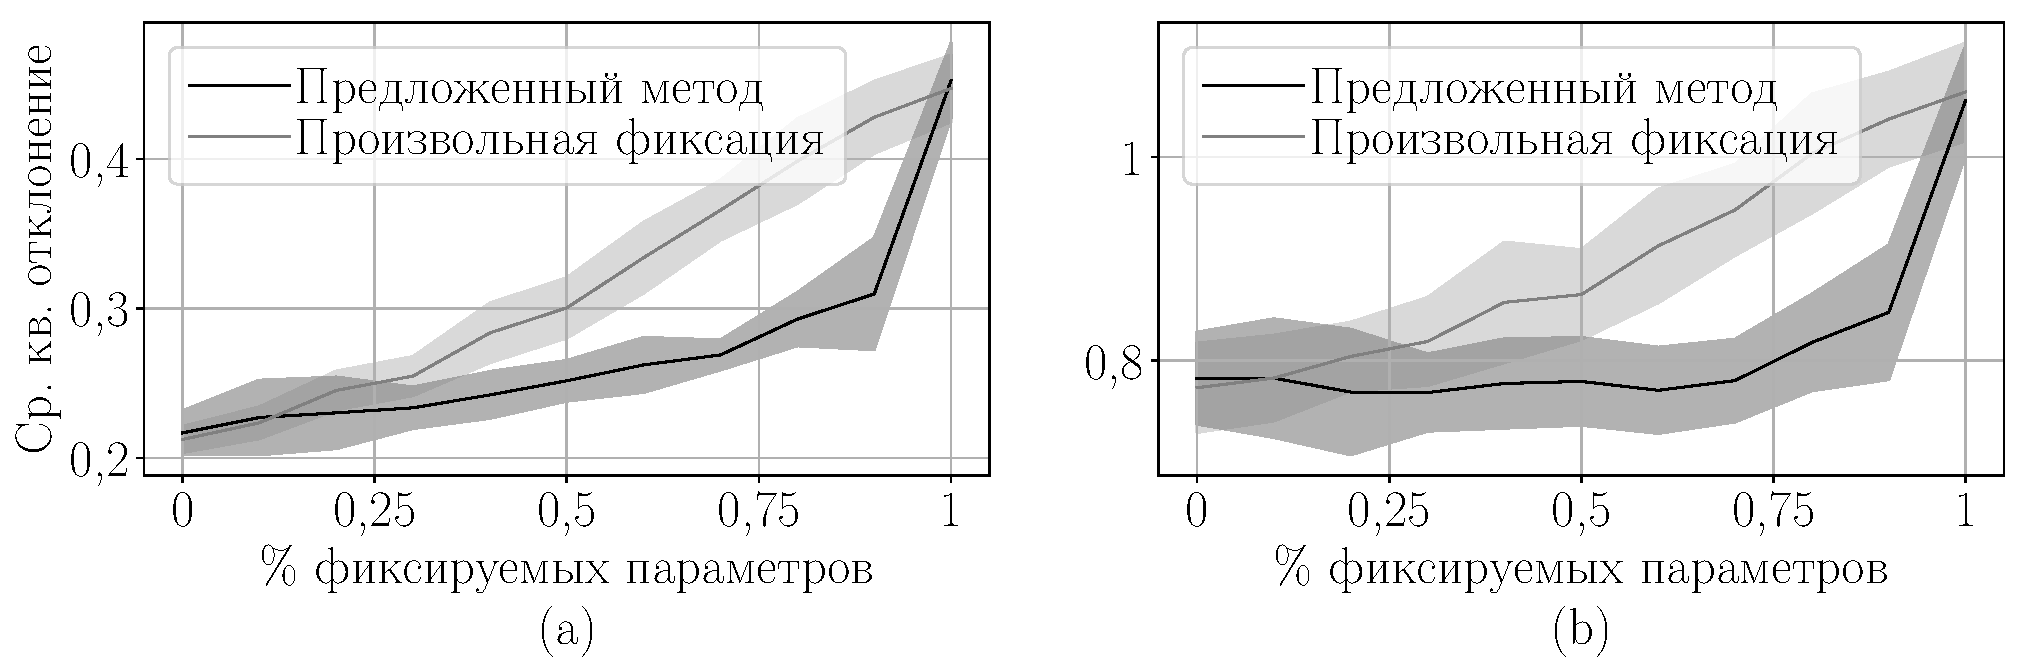
\includegraphics[width=1\textwidth]{results/order/generate_data_neural_loss}
\caption{Зависимость качества модели от числа зафиксированных параметров: a) на обучающей выборке; b) на тестовой выборке}
\label{fg:ex:syn3:1}
\end{figure}

\begin{figure}[h!t]\center
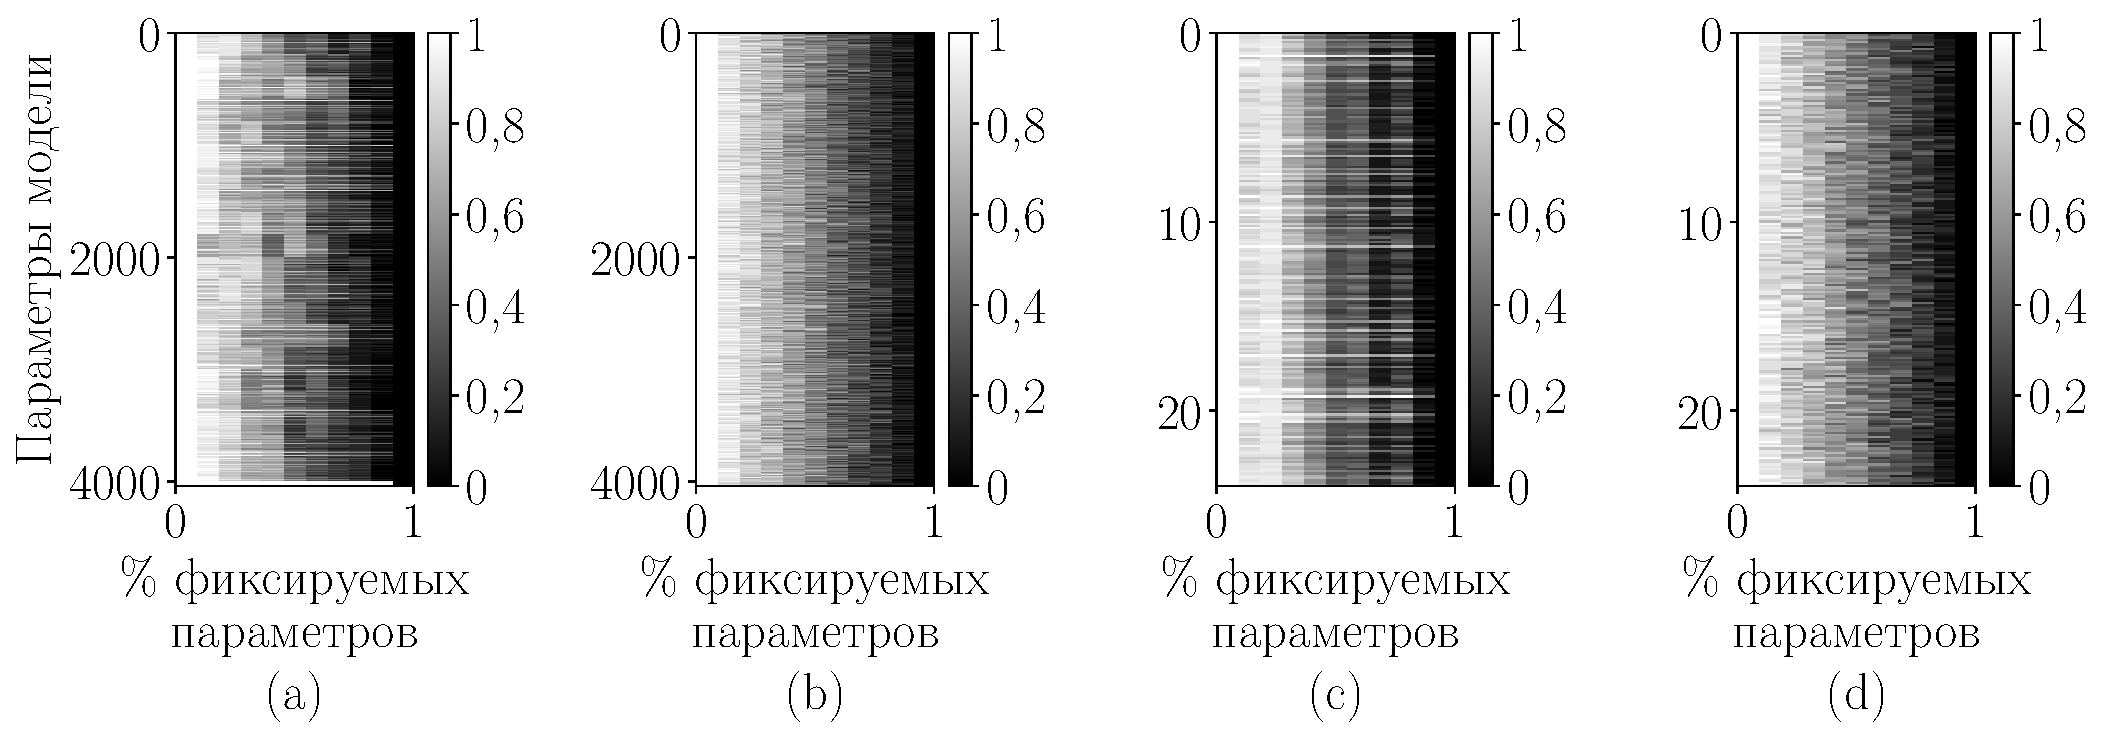
\includegraphics[width=1\textwidth]{results/order/generate_data_neural_matshow}
\caption{Визуализация векторов $\hat{\bm{\alpha}}\bigr(k\bigr)$ в зависимости от числа фиксируемых параметров: a) все параметры модели упорядочены предложенным методом; b) все параметры модели упорядочены произвольным образом; c) часть параметров модели упорядочена предложенным методом; d) часть параметров модели упорядочена произвольным образом}
\label{fg:ex:syn3:2}
\end{figure}

Эксперимент проводился на синтетически построенных данных. В качестве модели использовалась двухслойная нейросеть --- перцептрон.
%На рис. \ref{fg:ex:syn3:1} показано, что фиксация параметров в соответствии с предложенным порядком является лучше, чем фиксация параметров произвольным образом, так как функция ошибки растет медленней при фиксации большего процента параметров.
На рис. \ref{fg:ex:syn3:1} показаны графики зависимости функции потерь $\mathcal{L}$ от числа фиксируемых параметров. В случае фиксации параметров предложенным методом функция потерь $\mathcal{L}$ растет медленней, чем в случае фиксации параметров произвольным образом.

На рис. \ref{fg:ex:syn3:2} показана зависимость векторов $\hat{\bm{\alpha}}\bigr(k\bigr)$ от числа фиксируемых параметров. Каждый столбец соответствует одному вектору $\hat{\bm{\alpha}}\bigr(k\bigr)$. На рис. \ref{fg:ex:syn3:2}a, \ref{fg:ex:syn3:2}с видно, что $\hat{\bm{\alpha}}\bigr(k\bigr)$ имеет большое число компонент вектора, близких к $1$. Так как $\hat{\bm{\alpha}}\bigr(k\bigr)$ является усреднением вектора с компонентами $0$ или $1$, то предложенный порядок задает некоторый устойчивый порядок на множестве параметров модели. На рис. \ref{fg:ex:syn3:2}b, \ref{fg:ex:syn3:2}d видно, что в случае произвольной фиксации параметров компоненты вектора $\hat{\bm{\alpha}}\bigr(k\bigr)$ имеют одинаковые значения, следовательно, никакого порядка на множестве параметров нет.

\paragraph{Выборка Boston Housing.}
\begin{figure}[h!t]\center
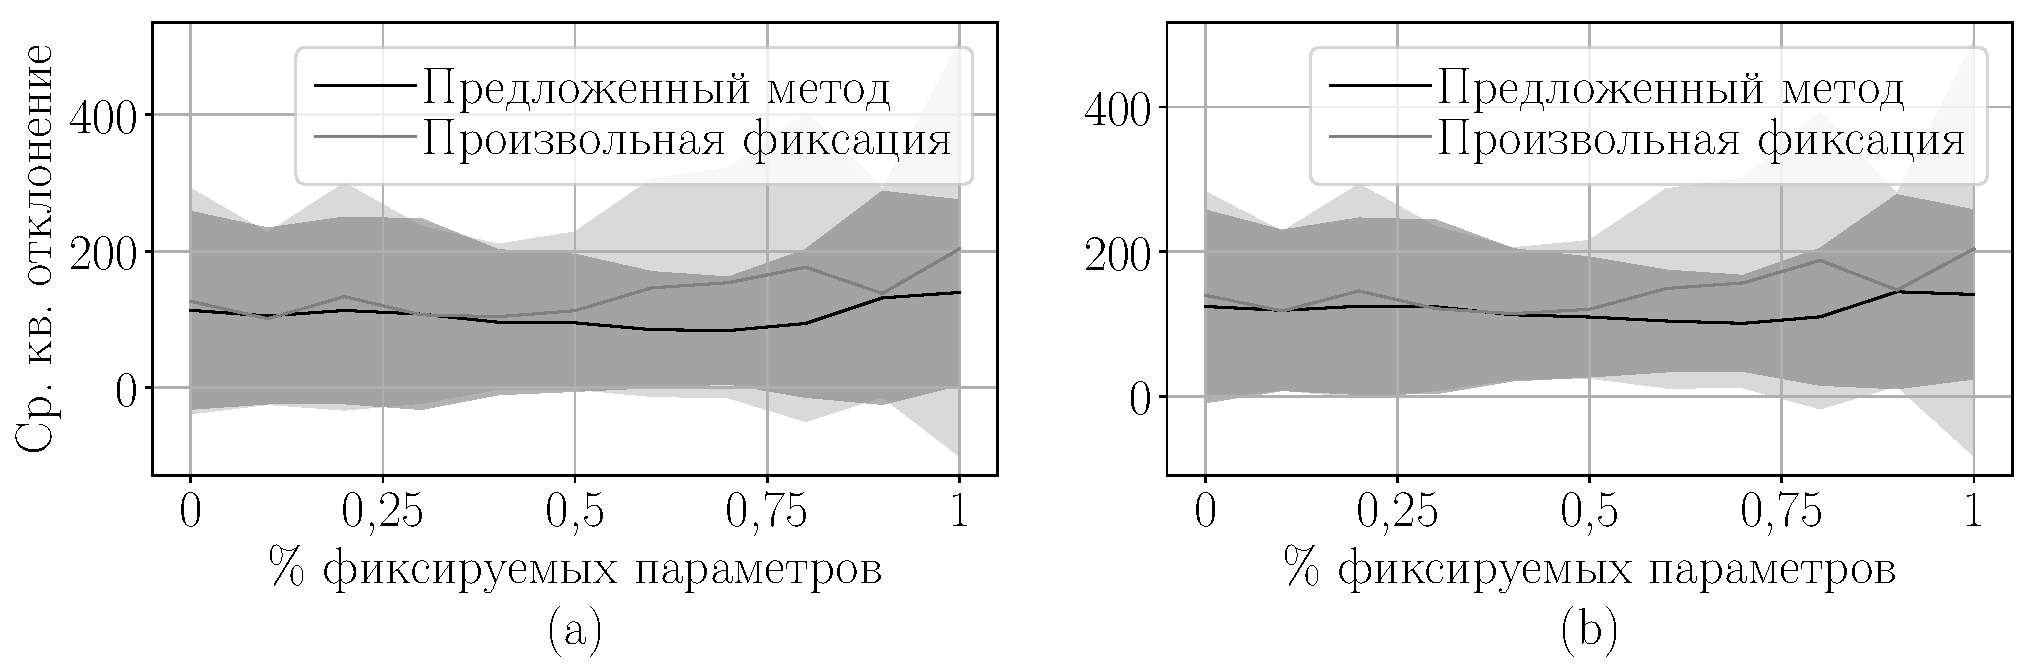
\includegraphics[width=1\textwidth]{results/order/boston_data_loss}
\caption{Зависимость качества модели от числа зафиксированных параметров: a) на обучающей выборке; b) на тестовой выборке}
\label{fg:ex:bost:1}
\end{figure}
Эксперимент проводился на реальных данных.
%На рис. \ref{fg:ex:bost:1} показано, что фиксация параметров в соответствии с предложенным порядком является лучше, чем заморозка параметров произвольным образом, так как функция ошибки растет медленней при фиксации параметров. Также видно, что в случае произвольной фиксации параметров функция ошибки имеет большую дисперсию, что указывает на сильную не устойчивость. Фиксация параметров предложенным методом является более устойчивым, что следует из того, что функция ошибки имеет меньше дисперсию.
На рис. \ref{fg:ex:bost:1} показаны графики зависимости функции потерь $\mathcal{L}$ от числа фиксируемых параметров. В случае фиксации параметров предложенным методом, функция потерь $\mathcal{L}$ растет так же, как и в случае фиксации параметров произвольным образом.
Данный результат следует из того, что нейросеть оказалась избыточно сложной моделью с большим числом параметров. После фиксации значимого числа параметров у модели оставалась большое число параметров для дообучения.

На рис. \ref{fg:ex:bost:2} показана зависимость векторов $\hat{\bm{\alpha}}\bigr(k\bigr)$ от числа фиксируемых параметров. На рис. \ref{fg:ex:bost:2}a, \ref{fg:ex:bost:2}с видно, что $\hat{\bm{\alpha}}\bigr(k\bigr)$ меняется незначительно от запуска к запуску алгоритма. Следовательно, предложенный порядок задает устойчивый к разным запускам порядок на множестве параметров модели. На рис. \ref{fg:ex:bost:2}b, \ref{fg:ex:bost:2}d видно, что в случае произвольной фиксации параметров вектор $\hat{\bm{\alpha}}\bigr(k\bigr)$ является произвольным и никакого порядка на множестве параметров нет.

\begin{figure}[h!t]\center
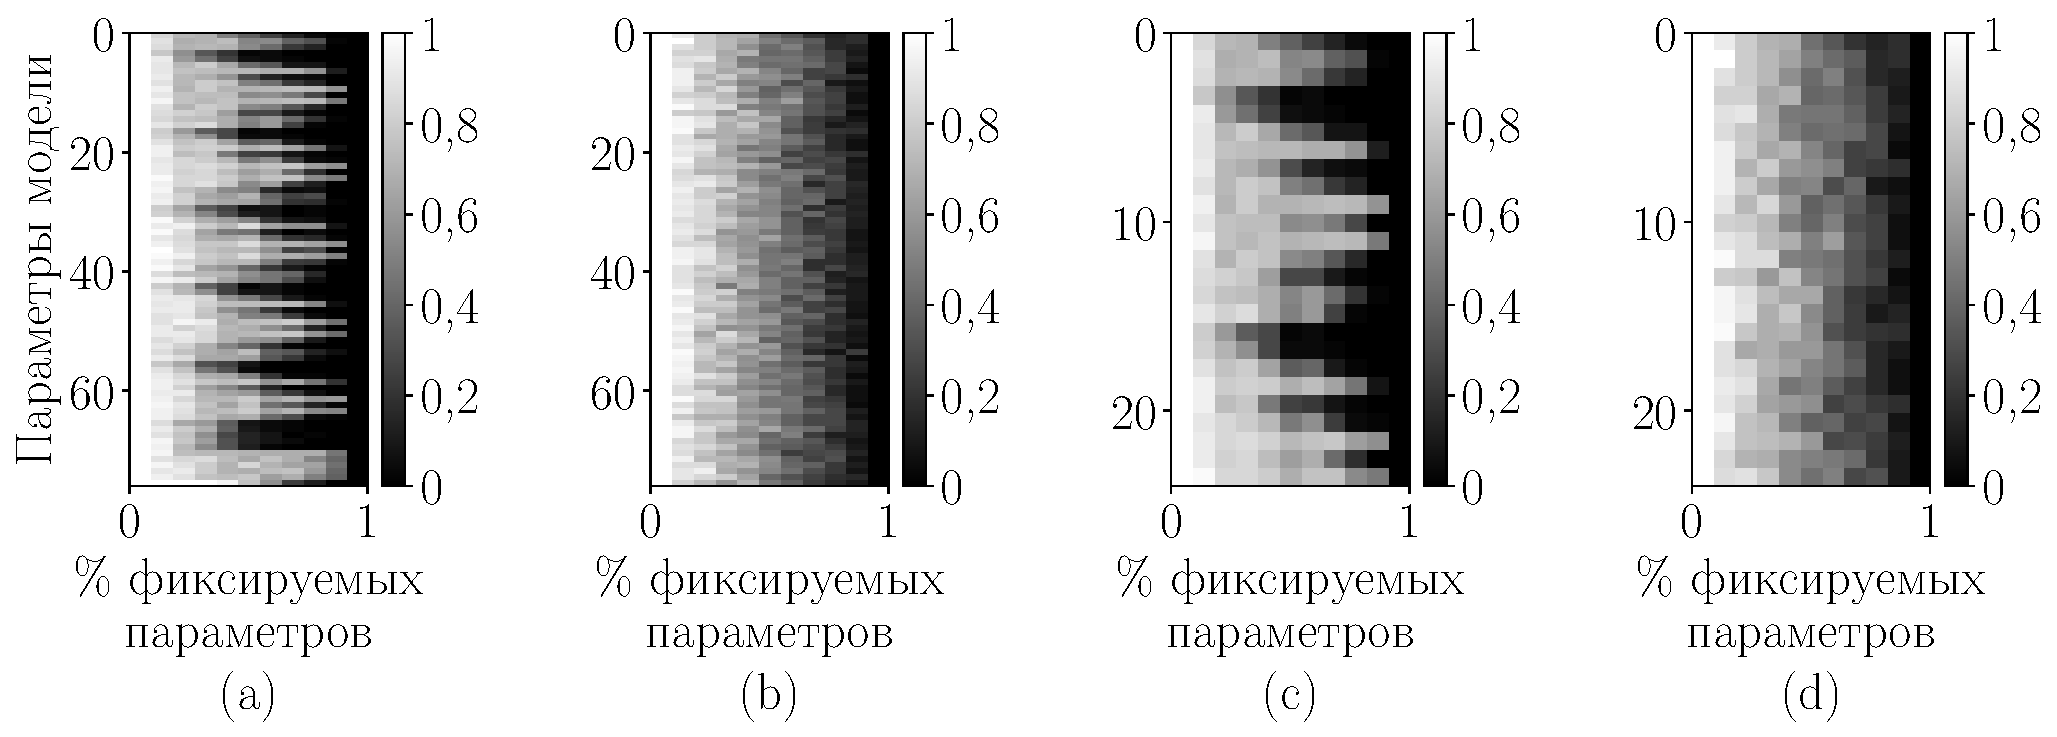
\includegraphics[width=1\textwidth]{results/order/boston_data_matshow}
\caption{Визуализация векторов $\hat{\bm{\alpha}}\bigr(k\bigr)$ в зависимости от числа фиксируемых параметров: a) все параметры модели упорядочены предложенным методом; b) все параметры модели упорядочены произвольным образом; c) часть параметров модели, упорядочена предложенным методом; d) часть параметров модели упорядочена произвольным образом}
\label{fg:ex:bost:2}
\end{figure}

\paragraph{Выборка Synthetic 3.}
\begin{figure}[h!t]\center
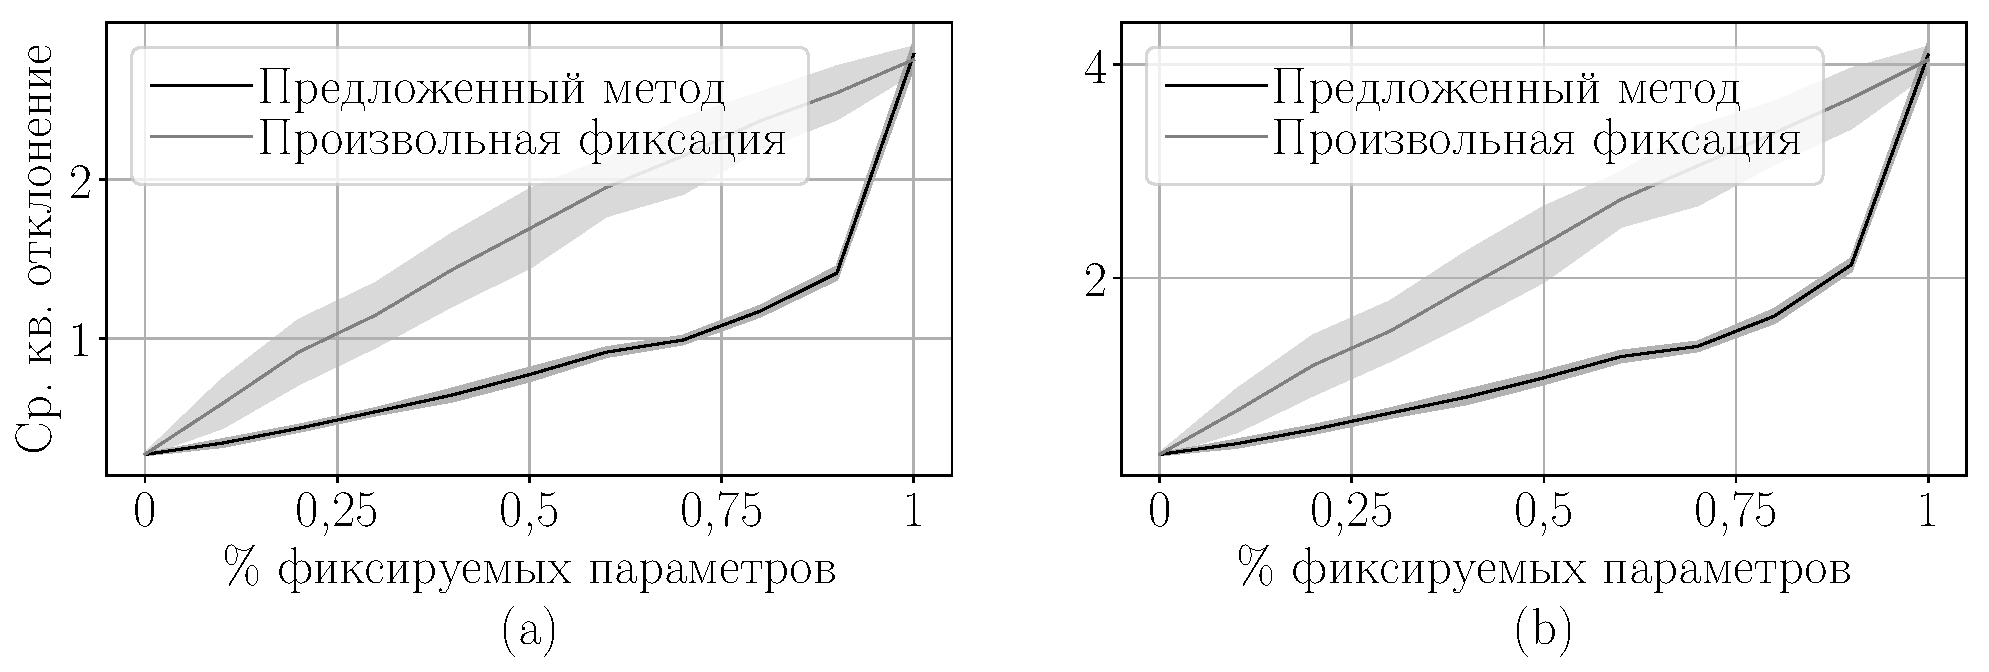
\includegraphics[width=1\textwidth]{results/order/generate_data_linear_loss}
\caption{Зависимость качества модели от числа зафиксированных параметров: a) на обучающей выборке; b) на тестовой выборке}
\label{fg:ex:syn1:1}
\end{figure}

\begin{figure}[h!t]\center
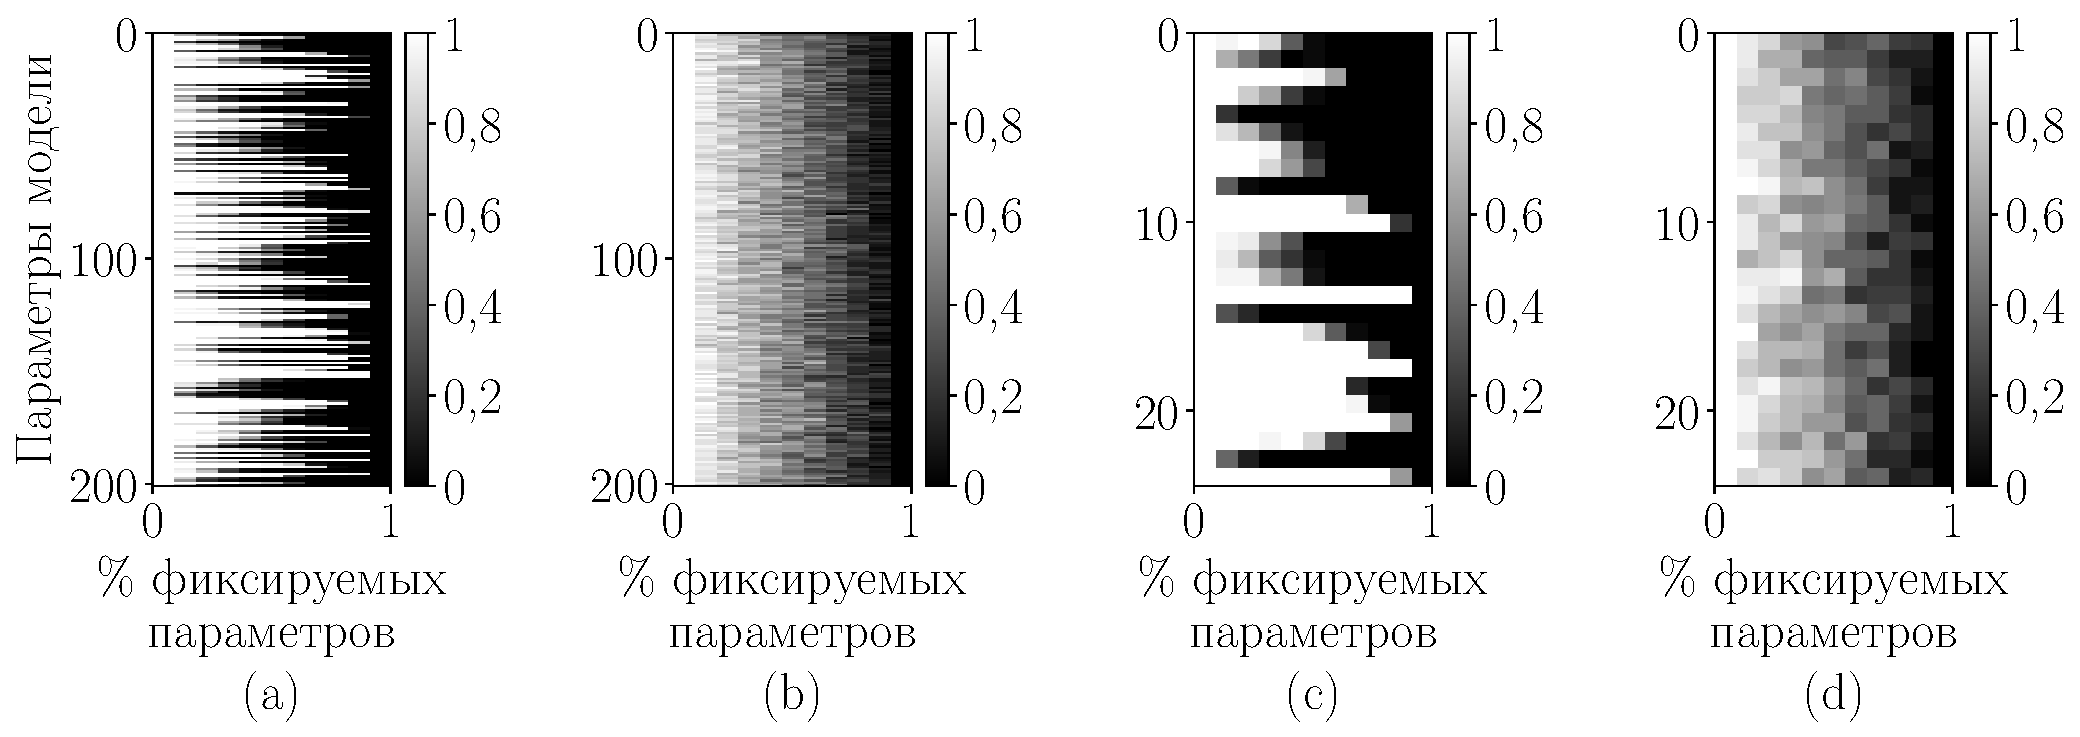
\includegraphics[width=1\textwidth]{results/order/generate_data_linear_matshow}
\caption{Визуализация векторов $\hat{\bm{\alpha}}\bigr(k\bigr)$ в зависимости от числа фиксируемых параметров: a) все параметры модели упорядочены предложенным методом; b) все параметры модели упорядочена произвольным образом; c) часть параметров модели, упорядочены предложенным методом; d) часть параметров модели упорядочена произвольным образом}
\label{fg:ex:syn1:2}
\end{figure}

Эксперимент проводился на синтетически построенных данных. В качестве модели использовалась линейная модель регрессии.
%На рис. \ref{fg:ex:syn1:1} показано, что фиксация параметров в соответсвии с предложенным порядком является лучше, чем фиксация параметров произвольным образом, так как функция ошибки растет медленней при фиксации параметров. Фиксация параметров предложенным методом является более устойчивым, что следует из того, что дисперсия функции ошибки почти отсутствует в отличии от дисперсии функции ошибки, где фиксация параметров производилась произвольным образом.
На рис. \ref{fg:ex:syn1:1} показаны графики зависимости функции потерь $\mathcal{L}$ от числа фиксируемых параметров. В случае фиксации параметров предложенным методом функция потерь $\mathcal{L}$ растет значительно медленней в сравнении со случаем фиксации параметров произвольным образом. Дисперсия функции ошибки также значительно меньше в случае фиксации параметров предложенным методом.

На рис. \ref{fg:ex:syn1:2} показано, что вектора $\hat{\bm{\alpha}}\bigr(k\bigr)$ не меняется от запуска к запуску. Так как данная модель линейная, то порядок на параметрах модели индуцирует некоторый порядок на множестве признаков.

\paragraph{Выборка MNIST.}

\begin{figure}[h!t]\center
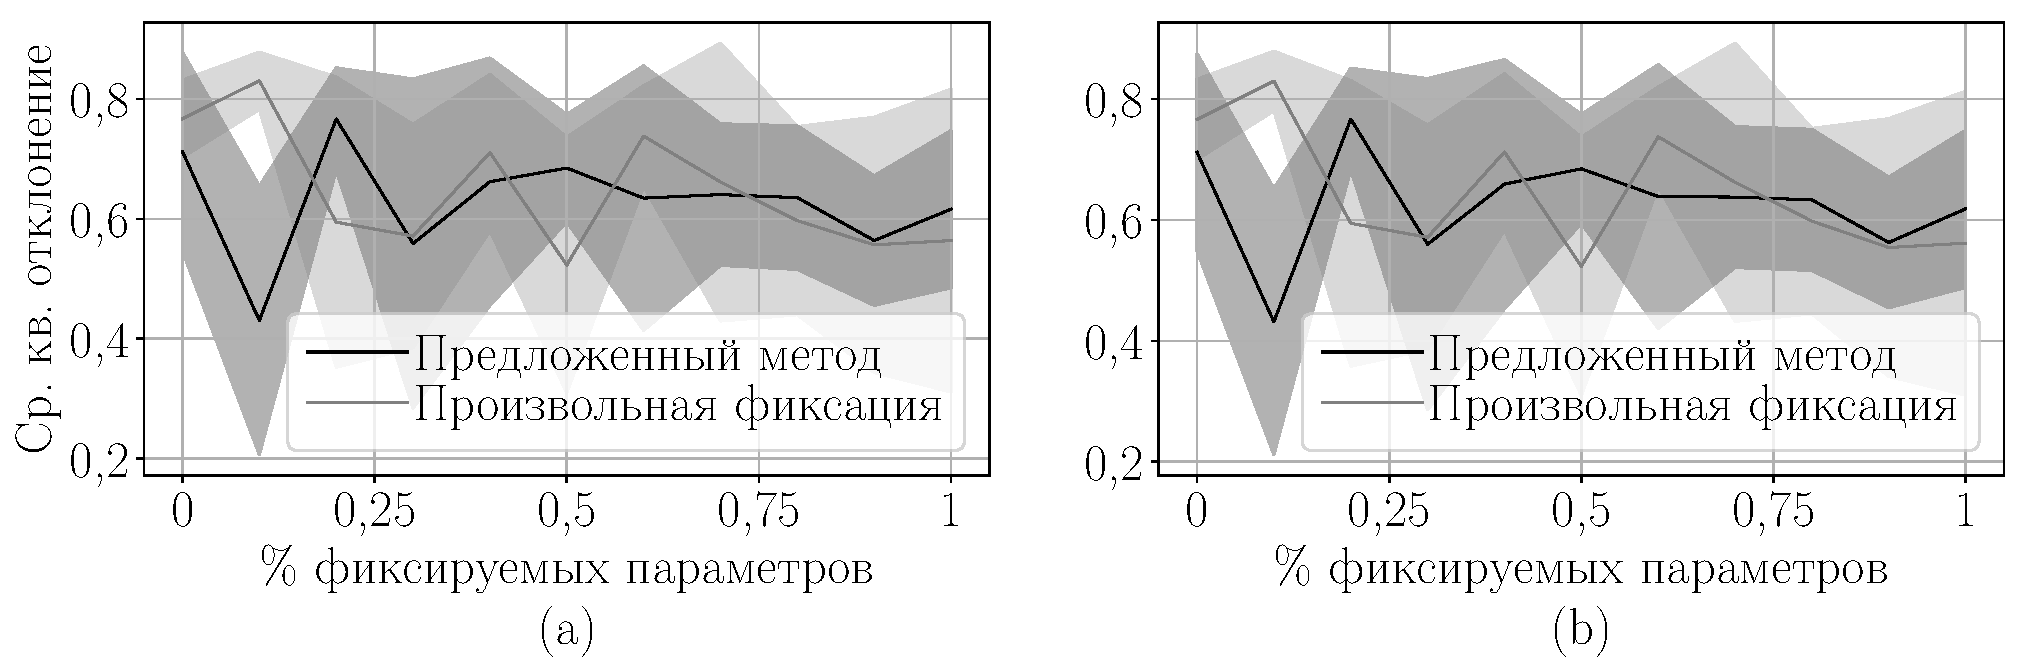
\includegraphics[width=1\textwidth]{results/order/mnist_data_loss}
\caption{Зависимость качества модели от числа зафиксированных параметров: a) на обучающей выборке; b) на тестовой выборке}
\label{fg:ex:mnist:1}
\end{figure}

\begin{figure}[h!t]\center
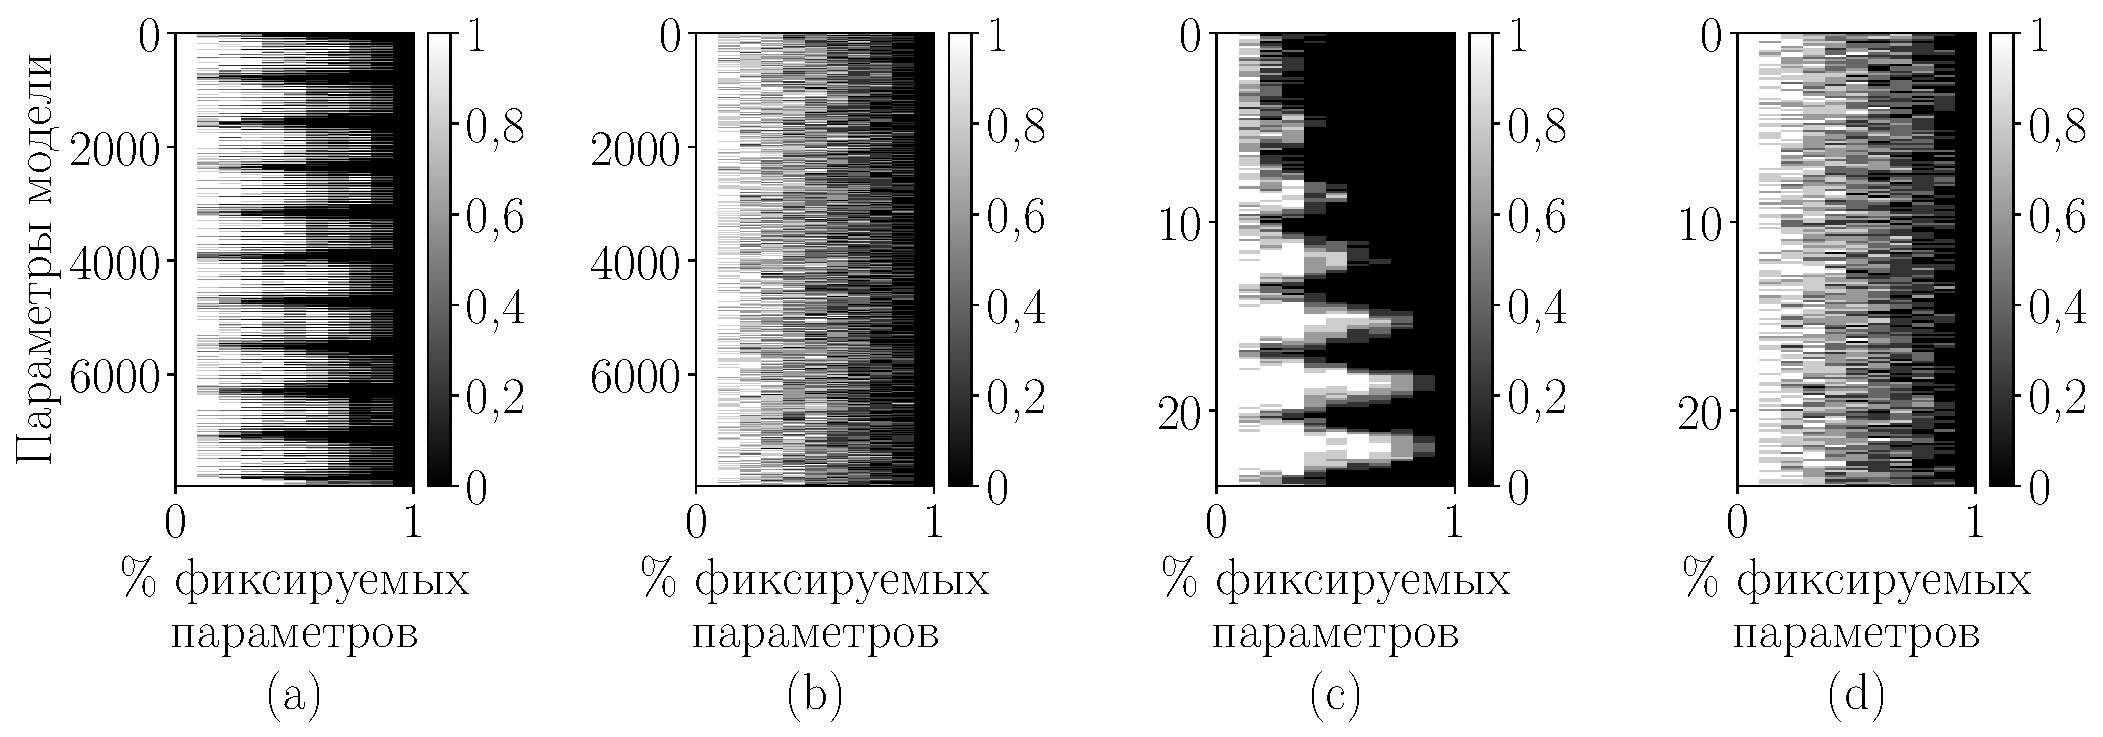
\includegraphics[width=1\textwidth]{results/order/mnist_data_matshow}
\caption{Визуализация векторов $\hat{\bm{\alpha}}\bigr(k\bigr)$ в зависимости от числа фиксируемых параметров: a) все параметры модели упорядочены предложенным методом; b) все параметры модели упорядочены произвольным образом; c) часть параметров модели упорядочена предложенным методом; d) часть параметров модели упорядочена произвольным образом}
\label{fg:ex:mnist:2}
\end{figure}

В эксперименте рассматривался двухслойный перцептрон для классификации изображений. В качестве входных данных рассматривались изображения размера $28\times28$, на которых изображены цифры. 

На рис. \ref{fg:ex:mnist:1} показано, что графики функции ошибки похожи в случае фиксации параметров параметров предложенным методом и в случае произвольной фиксации. Данный результат есть следствие того факта, что нейросеть является заведомо переусложненной моделью с большим числом параметров. После фиксации большого числа параметров у нейросети все еще остается значимое число параметров модели для дообучения.

На рис. \ref{fg:ex:mnist:2} показано, что в случае модели со значимым числом оптимизационных параметров,предложенный метод упорядочения параметров устойчив от запуску к запуску.




% Выводы
\newpage

\section{Заключение}
В рамках данного реферата приведен обзор существующих подходов для снижения сложности моделей глубокого обучения. Снижения сложности моделей глубокого обучения производится с целью улучшения интерпретируемости моделей глубокого обучения.

Рассмотрена проблема задания порядка на множестве параметров сложных аппроксимирующих моделей. Исследован метод задания порядка на основе анализа стохастических свойств градиента функции ошибки $\mathcal{L}$ по параметрам модели. Для задания порядка использовалась ковариационная матрица градиентов параметров~$\textbf{C}_{\eta_0}$, которая рассчитывается итеративно, в течение $t_0$ итераций градиентного метода параллельно оптимизации. Число итераций~$t_0$ выбиралось заранее экспериментально. Отдельно стоит заметить, что данный метод позволяет упорядочивать параметры в процессе оптимизации параметров модели. Также рассмотрены методы оптимального прореживания, метод основаный на вариационном подходе, а также метод основанный на методе Белсли для удаления зависимых параметров модели. Все данные методы позволяет задать полный порядок на множестве параметров моделей глубокого обучения. 

Полный порядок на множестве параметров позволяет выбирать архитектуры нейросетевых моделей ученика. Выбранные архитектуры рассматриваются в качестве модели ученика в методах дистилляции.

% Библиографические ссылки
\newpage

\setcounter{secnumdepth}{0}
\section{Список литературы}
\begingroup
\renewcommand{\section}[2]{}%
\begin{thebibliography}{10}
\bibitem{cifar10}
	\textit{Alex Krizhevsky and Vinod Nair and Geoffrey Hinton} CIFAR-10 (Canadian Institute for Advanced Research) // \url{http://www.cs.toronto.edu/~kriz/cifar.html}
\bibitem{imagenet}
	\textit{Deng, J., Dong, W., Socher, R., Li, L.-J., Li, K., Fei-Fei, L. } Imagenet: A large-scale hierarchical image database //  IEEE conference on computer vision and pattern recognition, 2009. P. 248--255. 
	
\bibitem{Zehao2017}
	\textit{{Huang}, Zehao and {Wang}, Naiyan} Like What You Like: Knowledge Distill via Neuron Selectivity Transfer // arXiv e-prints, 2017.
\bibitem{Wine}
	\textit{S. Aeberhard} Wine Data Set, 1991.
\bibitem{Zheng2020}
	\textit{Kui Ren and Tianhang Zheng and Zhan Qin and Xue Liu} Adversarial Attacks and Defenses in Deep Learning // Engineering, 2020. P. 346--360.
\bibitem{Krizhevsky2012}
	\textit{Alex Krizhevsky, Ilya Sutskever, Geoffrey Hinton} ImageNet Classification with Depp Convolutional Neural Networks // NIPS, 2012.
\bibitem{Simonyan2014}
	\textit{Karen Simonyan and Andrew Zisserman} Very Deep Convolutional Networks for Large-Scale Image Recognition // NIPS, 2014.
\bibitem{Vaswani2017}
	\textit{Vaswani A., Shazeer N., Parmar N., Uszkoreit J., Jones L., Gomez A., Kaiser L., Polosukhin I.} Attention Is All You Need // In Advances in Neural Information Processing Systems. 2017. V. 5. P. 6000--6010.
\bibitem{Devlin2018}
       \textit{Devlin J., Chang M., Lee K., Toutanova K.} BERT: Pre-training of Deep Bidirectional Transformers for Language Understanding // arXiv preprinted, 2018.
\bibitem{Brown2020}
        \textit{Tom B. Brown et al} GPT3: Language Models are Few-Shot Learners // arXiv preprinted, 2020.
\bibitem{Linting2021}
        \textit{Linting Xue and Noah Constant and Adam Roberts and Mihir Kale and Rami Al-Rfou and Aditya Siddhant and Aditya Barua and Colin Raffel.} mT5: A massively multilingual pre-trained text-to-text transformer // arXiv preprinted, 2021.
\bibitem{Ziqing2020}
        \textit{Yang, Ziqing and Cui, Yiming and Chen, Zhipeng and Che, Wanxiang and Liu, Ting and Wang, Shijin and Hu, Guoping} {T}ext{B}rewer: {A}n {O}pen-{S}ource {K}nowledge {D}istillation {T}oolkit for {N}atural {L}anguage {P}rocessing // Proceedings of the 58th Annual Meeting of the Association for Computational Linguistics: System Demonstrations.  2020. P. 9--16.
\bibitem{Kaiming2015}
	\textit{He K., Zhang X., Ren S., Sun J.} Deep Residual Learning for Image Recognition // Proc. of the IEEE Conference on Computer Vision and Pattern Recognition. Las Vegas, 2016. P. 770--778.
\bibitem{bachteev2018}
	\textit{Бахтеев О.\,Ю., Стрижов В.\,В.} Выбор моделей глубокого обучения субоптимальной сложности // АиТ. 2018. № 8. С. 129--147.
\bibitem{Hinton2015}
        \textit{Hinton G., Vinyals O., Dean J.} Distilling the Knowledge in a Neural Network // NIPS Deep Learning and Representation Learning Workshop. 2015.
\bibitem{mnist}
	\textit{LeCun Y.,  Cortes C., Burges C.} The MNIST dataset of handwritten digits, 1998. \text{http://yann.lecun.com/exdb/mnist/index.html}.
\bibitem{Vapnik2015}
	\textit{Vapnik V., Izmailov R.} Learning Using Privileged Information: Similarity Control and Knowledge Transfer // Journal of Machine Learning Research. 2015. No 16. P. 2023--2049.
\bibitem{Lopez2016}
	\textit{Lopez-Paz D., Bottou L., Scholkopf B., Vapnik V.} Unifying Distillation and Privileged Information // In International Conference on Learning Representations. Puerto Rico, 2016.
\bibitem{Ivakhnenko1994}
	\textit{Madala H., Ivakhnenko A.} Inductive Learning Algorithms for Complex Systems Modeling. Boca Raton: CRC Press Inc., 1994.
\bibitem{fashionmnist}
	\textit{Xiao H., Rasul K.,Vollgraf R.} Fashion-MNIST: a Novel Image Dataset for Benchmarking Machine Learning Algorithms // arXiv preprint arXiv:1708.07747. 2017.
\bibitem{twiter2013}
	\textit{Wilson T., Kozareva Z., Nakov P., Rosenthal S., Stoyanov V., Ritter A.} {S}em{E}val-2013 Task 2: Sentiment Analysis in Twitter // Proceedings of the Seventh International Workshop on Semantic Evaluation ({S}em{E}val 2013). Atlanta, 2013. P. 312--320.
\bibitem{LeCun1989}
	\textit{LeCun Y., Boser B., Denker J., Henderson D., Howard R., Hubbard W., Jackel L.} Backpropagation Applied to Handwritten Zip Code Recognition // Neural Computation. 1989. V. 1. No 4. P. 541--551.
\bibitem{Schmidhuber1997}
	\textit{Hochreiter S., Schmidhuber J.} Long short-term memory // Neural Computation. 1997. V. 9. No 8.  P. 1735--1780.
\bibitem{kingma2014}
	\textit{Kingma D, Ba J.} Adam: A Method for Stochastic Optimization // arXiv preprint arXiv:1412.6980. 2014.
\bibitem{graves2011}
	\textit{Graves A.} Practical Variational Inference for Neural Networks // Advances in Neural Information Processing Systems, 2011. Vol. 24. P. 2348--2356.
\bibitem{Vapnik2015}
	\textit{Vapnik V., Izmailov R.} Learning Using Privileged Information: Similarity Control and Knowledge Transfer // Journal of Machine Learning Research. 2015. No 16. P. 2023--2049.
\bibitem{Lopez2016}
	\textit{Lopez-Paz D., Bottou L., Scholkopf B., Vapnik V.} Unifying Distillation and Privileged Information // In International Conference on Learning Representations. Puerto Rico, 2016.
	
\bibitem{sutskever2014}
	\textit{Sutskever I., Vinyals O., Le Q.} Sequence to Sequence Learning with Neural Networks~// Advances in Neural Information Processing Systems, 2014. Vol.~2. P.~3104--3112.
	
\bibitem{Chunyan2016}
	\textit{Li C., Chen C., Carlson D., Carin L.} Preconditioned Stochastic Gradient Langevin Dynamics for Deep Neural Networks~// Thirtieth AAAI Conference on Artificial Intelligence.~---~Phoenix, USA, 2016. P.~1788--1794.
	
\bibitem{Tibshirani1996}
	\textit{Tibshirani R.} Regression shrinkage and selection via the Lasso~// Journal of the Royal Statistical Society, 1996. Vol.~58. P.~267--288.
	
\bibitem{Hastie2005}
	\textit{Zou H., Hastie T.} Regularization and variable selection via the Elastic Net~// Journal of the Royal Statistical Society, 2005. Vol.~67. P.~301--320.
	
\bibitem{srivastava2014}
	\textit{Srivastava N., Hinton G., Krizhevsky A., Sutskever I., Salakhutdinov R.} Dropout: A Simple Way to Prevent Neural Networks from Overfitting~// Journal of Machine Learning Research, 2014. Vol.~15. P.~1929--1958.
	
\bibitem{molchanov2017}
	\textit{Molchanov D., Ashukha A., Vetrov D.} Variational Dropout Sparsifies Deep Neural Networks~// 34th International Conference on Machine Learning.~---~Sydney, Australia, 2017. Vol.~70. P.~2498--2507.
	
\bibitem{cun1990}
	\textit{LeCun Y., Denker J., Solla S.} Optimal Brain Damage~// Advances in Neural Information Processing Systems, 1989. Vol.~2. P.~598--605.
	
\bibitem{grabovoy2019}
	\textit{Грабовой А. В., Бахтеев О. Ю., Стрижов В. В.} Определение релевантности параметров нейросети~// Информатика и ее применения, 2019. Т.~13. Вып.~2. С.~62--70.
\bibitem{grabovoy2020}
	\textit{Грабовой А. В., Бахтеев О. Ю., Стрижов В. В.} Введение отношения порядка на множестве параметров аппроксимирующих моделей~// Информатика и ее применения, 2019. Т.~14. Вып.~2. С.~58--65.

\bibitem{Mandt2017}
	\textit{Mandt S., Hoffman M., Blei D.} Stochastic Gradient Descent as Approximate Bayesian Inference~// Journal Of Machine Learning Research, 2017. Vol.~18. P.~1--35.
	
\bibitem{Kingma2014}
	\textit{Kingma D., Ba L.} Adam: A Method for Stochastic Optimization~// 3rd International Conference on Learning Representations.~---~San Diego, USA, 2015.

\bibitem{Boston}
	\textit{Harrison D.,  Rubinfeld D.} Hedonic prices and the demand for clean air~// Journal of Environmental Economics and Management, 1991. Vol.~5. P.~81--102.

\bibitem{mnist}
	\textit{LeCun Y.,  Cortes C., Burges C.} The MNIST dataset of handwritten digits, 1998. \url{http://yann.lecun.com/exdb/mnist/index.html}

\bibitem{maclarin2015}
	\textit{Maclaurin D.,  Duvenaud D., Adams R.} Gradient-based Hyperparameter Optimization Through Reversible Learning~// Proceedings of the 32th International Conference on Machine Learning, 2015. Vol.~37. P.~2113--2122.
\bibitem{luketina2015}
	\textit{Luketina J.,  Berglund M., Raiko T., Greff K.} Scalable Gradient-based Tuning of Continuous Regularization Hyperparameters~// Proceedings of the 33th International Conference on Machine Learning, 2016. Vol.~48. P.~2952--2960.
\bibitem{bishop2006}
	\textit{Bishop C.} Pattern Recognition and Machine Learning, 2006. Pp.~396.
\bibitem{neychev2016}
	\textit{Neychev R.,  Katrutsa A., Strijov V.} Robust selection of multicollinear features in forecasting~// Factory Laboratory, 2016. Vol.~82. P.~68--74.
\bibitem{cun1990}
	\textit{LeCun Y.,  Denker J., Solla S.} Optimal Brain Damage~// Advances in Neural Information Processing Systems, 1989. P.~598--605.
\bibitem{molchanov2017}
	\textit{Molchanov D.,  Ashukha A., Vetrov D.} Variational Dropout Sparsifies Deep Neural Networks~// Proceedings of the 34th International Conference on Machine Learning, 2017. Vol.~70. P.~2498--2507.
\bibitem{neal1995}
	\textit{Neal A.,  Radford M.} Bayesian Learning for Neural Networks, 1995.
\bibitem{sutskever2014}
	\textit{Sutskever I.,  Vinyals O., Le Q.} Sequence to Sequence Learning with Neural Networks, 2014. Vol.~2. P.~3104--3112.
\bibitem{graves2011}
	\textit{Graves A.} Practical Variational Inference for Neural Networks, 2011. P.~2348--2356.
\bibitem{louizos2017}
	\textit{Louizos C., Ullrich K., Welling M.} Bayesian Compression for Deep Learning, 2017. P.~3288--3298.

% series
\bibitem{kwapisz2010}
	\textit{J. R. Kwapisz, G. M. Weiss, S. A. Moore} Activity Recognition using Cell Phone Accelerometers~// Proceedings of the Fourth International Workshop on Knowledge Discovery from Sensor Data, 2010. Vol. 12. P. 74--82.
\bibitem{wang2014}
	\textit{W. Wang, H. Liu, L. Yu, F. Sun} Activity Recognition using Cell Phone Accelerometers~// Joint Conference on Neural Networks, 2014. P. 1185--1190.
\bibitem{Ignatov2015}
	\textit{A. D. Ignatov, V. V. Strijov} Human activity recognition using quasiperiodic time series collected from a single tri-axial accelerometer.~// Multimedial Tools and Applications, 2015.
\bibitem{Olivares2012}
	\textit{A. Olivares, J. Ramirez, J. M. Gorris, G. Olivares, M. Damas} Detection of (in)activity periods in human body motion using inertial sensors: A comparative study.~// Sensors, 12(5):5791–5814, 2012.
\bibitem{cinar2018}
	\textit{Y. G. Cinar and H. Mirisaee} Period-aware content attention RNNs for time series forecasting with missing values~// Neurocomputing, 2018. Vol. 312. P. 177--186.
\bibitem{motrenko2015}
	\textit{A. P. Motrenko, V. V. Strijov} Extracting fundamental periods to segment biomedical signals~// Journal of Biomedical and Health Informatics, 2015,~20(6). P.~1466~-~1476.
\bibitem{lukashin2003}
	\textit{Y. P. Lukashin} Adaptive methods for short-term forecasting~// Finansy and Statistik, 2003.
\bibitem{Ivkin2015}
	\textit{И. П. Ивкин,  М. П. Кузнецов} Алгоритм классификации временных рядов акселерометра по комбинированному признаковому описанию.~// Машинное обучение и анализ данных, 2015.
\bibitem{Katrutsa2015}
	\textit{V. V. Strijov, A. M. Katrutsa} Stresstes procedures for features selection algorithms.~// Schemometrics and Intelligent Laboratory System, 2015.
\bibitem{Borg2005}
	\textit{I. Borg, P. J. F. Groenen} Modern Multidimensional Scaling. --- New York: Springer, 2005. 540 p.
\bibitem{Shiglavsi1997}
	\textit{Д. Л. Данилова, А. А. Жигловский} Главные компоненты временных рядов: метод "Гусеница".~---~Санкт-Петербурскиий университет, 1997.
	
% priorexpert
\bibitem{Tianqi2016}
	\textit{Tianqi~C., Carlos~G.} XGBoost: A Scalable Tree Boosting System~// Proceedings of the 22nd ACM SIGKDD International Conference on Knowledge Discovery and Data Mining. 2016.
\bibitem{Ishwaran2012}
	\textit{Xi~C., Hemant~I.} Random Forests for Genomic Data Analysis~// Genomics. 2012. Issues.~99. \No~6. P.~323--329.
\bibitem{Yuksel2012}
	\textit{Esen~Y.\,S., Wilson~J., Gader~P.\,D.} Twenty Years of Mixture of Experts~// IEEE Transactions on Neural Networks and Learning Systems. 2012. Issues.~23. \No~8. P.~1177--1193.
\bibitem{Edward2002}
	\textit{Rasmussen~C.\,E., Ghahramani~Z.} Infinite Mixtures of Gaussian Process Experts~// Advances in Neural Information Processing Systems 14. 2002. P.~881--888.
\bibitem{Shazeer2017}
	\textit{Shazeer~N., Mirhoseini~A., Maziarz~K.} Outrageously large neural networks: the sparsely-gated mixture-of-experts layer~//  International Conference on Learning Representations. 2017.
\bibitem{Jordan1994}
	\textit{Jordan~M.\,I.} Hierarchical mixtures of experts and the EM algorithm~// Neural Comput. 1994. Vol.~6, \No~2. P.~181--214.
\bibitem{Jordan1991}
	\textit{Jordan~M.\,I., Jacobs~R.\,A.} Hierarchies of adaptive experts~// In Advances in Neural Information Processing Systems. 1991. P.~985--992.
\bibitem{Lima2007}
	\textit{Lima~C., Coelho~A., Zuben~F.\,J.} Hybridizing mixtures of experts with support vector machines: Investigation into nonlinear dynamic systems identification~// Inf. Sci. 2007. Vol.~177. \No~10. P.~2049--2074.
\bibitem{Cao2003}
	\textit{Cao~L.} Support vector machines experts for time series forecasting~// Neurocomputing. 2003. Vol.~51. P.~321--339.
\bibitem{Yumlu2003}
	\textit{Yumlu~M.\,S., Gurgen~F.\,S.,  Okay~N.} Financial time series prediction using mixture of experts~// In Proc. 18th Int. Symp. Comput. Inf. Sci. 2003. P.~553--560.
\bibitem{Cheung1995}
	\textit{Cheung~Y.\,M., Leung~W.\,M., Xu~L.} Application of mixture of experts model to financial time series forecasting~// On Proc. Int. Conf. Neural Netw. Signal Process. 1995. P.~1--4.
\bibitem{Weigend2000}
	\textit{Weigend~A.\,S., Shi~S.} Predicting daily probability distributions of S\&P500 returns~// J. Forecast. 2000. Vol.~19. \No~4. P.~375--392.
\bibitem{Ebrahimpour2009}
	\textit{Ebrahimpour~R., Moradian~M.\,R., Esmkhani~A., Jafarlou~F.\,M.} Recognition of Persian handwritten digits using characterization loci and mixture of experts~// J. Digital Content Technol. Appl. 2009. Vol.~3. \No~3. P.~42--46.
\bibitem{Estabrooks2001}
	\textit{Estabrooks~A., Japkowicz~N.} A mixture-of-experts framework for text classification~//In Proc. Workshop Comput. Natural Lang. Learn., Assoc. Comput. Linguist. 2001. P.~1--8.
\bibitem{Mossavat2010}
	\textit{Mossavat~S., Amft~O., Petkov~Vries~B., Kleijn~W.} A Bayesian hierarchical mixture of experts approach to estimate speech quality~// In Proc. 2nd Int. Workshop Qual. Multimedia Exper. 2010. P.~200--205.
\bibitem{Peng1996}
	\textit{Peng~F., Jacobs~R.\,A., Tanner~M.\,A.} Bayesian inference in mixtures-of-experts and hierarchical mixtures-of-experts models with an application to speech recognition~// J. Amer. Stat. Assoc. 1996. Vol.~91. \No~435. P. 953--960.
\bibitem{Tuerk2001}
	\textit{Tuerk~A.} The state based mixture of experts HMM with applications to the recognition of spontaneous speech. Ph.D. thesis. Cambridge: Univ. Cambridge, 2001.
\bibitem{Sminchisescu2007}
	\textit{Sminchisescu~C., Kanaujia~A., Metaxas~D.} Discriminative density propagation for visual tracking~// IEEE Trans. Pattern Anal. Mach. Intell. 2007. Vol.~29. \No~11. P. 2030--2044.
\bibitem{Bowyer2010}
	\textit{Bowyer~K., Hollingsworth~K., Flynn~P.} A Survey of Iris Biometrics Research: 2008--2010.
\bibitem{Matveev2010}
	\textit{Matveev~I.} Detection of iris in image by interrelated maxima of brightness gradient projections~// Appl.Comput. Math. 2010. Vol.~9. \No~2. P. 252--257.
\bibitem{Matveev2014}
	\textit{Matveev~I., Simonenko~I.}. Detecting precise iris boundaries by circular shortest path method~// Pattern Recognition and Image Analysis. 2014. Vol. 24. P. 304--309.
\bibitem{Dempster1977}
	\textit{Dempster~A.\,P., Laird~N.\,M., Rubin~D.\,B.} Maximum Likelihood from Incomplete Data via the EM Algorithm~// Journal of the Royal Statistical Society. Series B (Methodological). 1977. Vol. 39. \No~1 P. 1--38.
\bibitem{bishop2006}
	\textit{Bishop~C.} Pattern Recognition and Machine Learning. Berlin: Springer, 2006. P. 758.
	
% Bazarova
\bibitem{Akhtar2018}
	Akhtar N, Mian A (2018) Threat of Adversarial Attacks on Deep Learning in Computer Vision: A Survey. IEEE Access 6:14410--14430
\bibitem{bishop2006}
	Bishop C. (2010) Pattern Recognition and Machine Learning. Springer, Berlin 
\bibitem{Bowyer2010}
	Bowyer K, Hollingsworth K, Flynn P (2010) A Survey of Iris Biometrics Research: 2008-2010. Handbook of iris recognition 15--54
\bibitem{Cao2003}
	Cao L (2003) Support vector machines experts for time series forecasting. Neurocomputing 51:321--339
\bibitem{Tianqi2016}
	Chen T, Guestrin C (2016) XGBoost: A Scalable Tree Boosting System. KDD ’16 Proceedings of the 22nd ACM SIGKDD International Conference on Knowledge Discovery and Data Mining 785--794
\bibitem{Ishwaran2012}
	Chen Xi, Ishwaran H (2012) Random Forests for Genomic Data Analysis. Genomics 6:323--329
\bibitem{Cheung1995}
	Cheung Y, Leung W, Xu L (1995) Application of mixture of experts model to financial time series forecasting. In Proc. Int. Conf. Neural Netw. Signal Process. 1--4
\bibitem{Dempster1977}
	Dempster A, Laird N, Rubin D (1997) Maximum Likelihood from Incomplete Data via the EM Algorithm. Journal of the Royal Statistical Society. Series B (Methodological) 39:1--38
\bibitem{Estabrooks2001}
	Estabrooks A, Japkowicz N (2001) A mixture-of-experts framework for text classification. In Proc. Workshop Comput. Natural Lang. Learn., Assoc. Comput. Linguist. 1--8
\bibitem{Ebrahimpour2009}
	Ebrahimpour R, Moradian R, Esmkhani A, Jafarlou F (2009) Recognition of Persian handwritten digits using characterization loci and mixture of experts. J. Digital Content Technol. Appl. 42--46
\bibitem{Han2020}
	Han X, Yao M, Debayan D, Hui L, Ji-Liang T, Anil J (2020) Adversarial Attacks and Defenses in Images, Graphs and Text: A Review. International Journal of Automation and Computing 17:151--178
\bibitem{Kaiming2015}
	Kaiming H, Xiangyu Z, Shaoqing R, Jian S (2016) Deep Residual Learning for Image Recognition. Proceedings of the IEEE Conference on Computer Vision and Pattern Recognition 770--778
\bibitem{Matveev2010}
	Matveev I (2010) Detection of iris in image by interrelated maxima of brightness gradient projections. Appl. Comput. Math 9:252--257
\bibitem{Matveev2014}
	Matveev I, Simonenko I (2014) Detecting precise iris boundaries by circular shortest path method. Pattern Recognition and Image Analysis 24:304--309
\bibitem{Mossavat2010}
	Mossavat S, Amft O, Vries B, Petkov P, Kleijn W (2010) A Bayesian hierarchical mixture of experts approach to estimate speech quality. In Proc. 2nd Int. Workshop Qual. Multimedia Exper. 200--205
\bibitem{Peng1996}
	Peng F, Jacobs R, Tanner M (1996) Bayesian inference in mixtures-of-experts and hierarchical mixtures-of-experts models with an application to speech recognition. J. Amer. Stat. Assoc. 91:953--960
\bibitem{Ribeiro2016}
	Ribeiro M, Singh S, Guestrin C (2016) Why Should I Trust You?": Explaining the Predictions of Any Classifier. KDD ’16 Proceedings of the 22nd ACM SIGKDD International Conference on Knowledge Discovery and Data Mining 1135--1144
\bibitem{Dalila2018}
	Salamani D, Gadatsch S, Golling T,  Stewart G, Ghosh A,  Rousseau D,  Hasib A,  Schaarschmidt J (2018) Deep Generative Models for Fast Shower Simulation in ATLAS. 2018 IEEE 14th International Conference on e-Science (e-Science) \text{https://doi.org/10.1109/eScience.2018.00091}
\bibitem{Sminchisescu2007}
	Sminchisescu C, Kanaujia A, Metaxas D (2007) Discriminative density propagation for visual tracking. IEEE Trans. Pattern Anal. Mach. Intell. 29:2030--2044
\bibitem{Tuerk2001}
	Tuerk A (2001) The state based mixture of experts HMM with applications to the recognition of spontaneous speech. Ph.D. thesis, University of Cambridge.
\bibitem{Weigend2000}
	Weigend A, Shi S (2000) Predicting daily probability distributions of S\&P500 returns. J. Forecast 19:375--392
\bibitem{Yuksel2012}
	Yuksel S, Wilson J, Gader P (2012) Twenty Years of Mixture of Experts. IEEE Transactions on Neural Networks and Learning Systems 8:1177--1193
\bibitem{Yumlu2003}
	Yumlu M, Gurgen F,  Okay N (2003) Financial time series prediction using mixture of experts. In Proc. 18th Int. Symp. Comput. Inf. Sci. 553--560

% samplesize
\bibitem{demidenko2007}
	Demidenko E (2007) Sample size determination for logistic regression revisited. \textit{Statist. Med.} 26:3385--3397.
\bibitem{boston}
	Harrison D, Rubinfeld D (1978) Hedonic prices and the demand for clean air. \textit{Economics and Management} 5:81--102.
\bibitem{joseph1997}
	Joseph L, Berger R, Be'lisle P (1995) Bayesian and mixed bayesian likelihood criteria for sample size determination. \textit{Statistician} 16:769--781.
\bibitem{joseph1995}
	Joseph L, Wolfson D, Berger R (1997) Sample size calculations for binomial proportions via highest posterior density intervals. \textit{Statistical Medicine} 44:143--154.
\bibitem{kloek1975}
	Kloek T (1975). Note on a large-sample result in specification analysis. \textit{Econometrica} 43:933--936.
\bibitem{lindley1997}
	Lindley D (1997) The choice of sample size. \textit{The Statistician} 46:129--138.
\bibitem{motrenko2014}
	Motrenko A, Strijov V, Weber G (2014) Sample size determination for logistic regression. \textit{Journal of Computational and Applied Mathematics} 255:743--752.
\bibitem{servo}
	Quinlan J (1992) Learning with continuous classes. \textit{Proc. 5th Australian Joint Conference on AI} 343--348.
\bibitem{qumsiyeh2013}
	Qumsiyeh M (2013) Using the bootstrap for estimation the sample size in statistical experiments. \textit{Journal of modern applied statistical methods} 8:305--321.
\bibitem{rubin1998}
	Rubin D, Stern H (1998) Sample size determination using posterior predictive distributions. \textit{Sankhya: The Indian Journal of Statistics Special Issue on Bayesian Analysis} 60:161--175.
\bibitem{self1988}
	Self S, Mauritsen R (1988) Power/sample size calculations for generalized linear models. \textit{Biometrics} 44:79--86.
\bibitem{self1992}
	Self S, Mauritsen R, Ohara J (1992) Power calculations for likelihood ratio tests in generalized linear models. \textit{Biometrics} 48:31--39.
\bibitem{shieh2000}
	Shieh G (2000) On power and sample size calculations for likelihood ratio tests in generalized linear models. \textit{Biometrics} 56:1192--1196.
\bibitem{shieh2005}
	Shieh G (2005) On power and sample size calculations for Wald tests in generalized linear models. \textit{Journal of Statistical Planning and Inference} 128:43--59.
\bibitem{wang2002}
	Wang F, Gelfand A (2002) A Simulation-based Approach to Bayesian Sample Size Determination for Performance under a Given Model and for Separating Models. \textit{Statistical Science} 17:193--208.
	
% priveleage learning
\bibitem{Vaswani2017}
	\textit{Vaswani A., Shazeer N., Parmar N., Uszkoreit J., Jones L., Gomez A., Kaiser L., Polosukhin I.} Attention Is All You Need // In Advances in Neural Information Processing Systems. 2017. V. 5. P. 6000--6010.
\bibitem{Devlin2018}
	\textit{Devlin J., Chang M., Lee K., Toutanova K.} BERT: Pre-training of Deep Bidirectional Transformers for Language Understanding // arXiv preprint arXiv:1810.04805. 2018.
\bibitem{Kaiming2015}
	\textit{He K., Zhang X., Ren S., Sun J.} Deep Residual Learning for Image Recognition // Proc. of the IEEE Conference on Computer Vision and Pattern Recognition. Las Vegas, 2016. P. 770--778.
\bibitem{bachteev2018}
	\textit{Бахтеев О.\,Ю., Стрижов В.\,В.} Выбор моделей глубокого обучения субоптимальной сложности // АиТ. 2018. № 8. С. 129--147.
\bibitem{Hinton2015}
        \textit{Hinton G., Vinyals O., Dean J.} Distilling the Knowledge in a Neural Network // NIPS Deep Learning and Representation Learning Workshop. 2015.
\bibitem{mnist}
	\textit{LeCun Y.,  Cortes C., Burges C.} The MNIST dataset of handwritten digits, 1998. \text{http://yann.lecun.com/exdb/mnist/index.html}.
\bibitem{Vapnik2015}
	\textit{Vapnik V., Izmailov R.} Learning Using Privileged Information: Similarity Control and Knowledge Transfer // Journal of Machine Learning Research. 2015. No 16. P. 2023--2049.
\bibitem{Lopez2016}
	\textit{Lopez-Paz D., Bottou L., Scholkopf B., Vapnik V.} Unifying Distillation and Privileged Information // In International Conference on Learning Representations. Puerto Rico, 2016.
\bibitem{Ivakhnenko1994}
	\textit{Madala H., Ivakhnenko A.} Inductive Learning Algorithms for Complex Systems Modeling. Boca Raton: CRC Press Inc., 1994.
\bibitem{fashionmnist}
	\textit{Xiao H., Rasul K.,Vollgraf R.} Fashion-MNIST: a Novel Image Dataset for Benchmarking Machine Learning Algorithms // arXiv preprint arXiv:1708.07747. 2017.
\bibitem{twiter2013}
	\textit{Wilson T., Kozareva Z., Nakov P., Rosenthal S., Stoyanov V., Ritter A.} {S}em{E}val-2013 Task 2: Sentiment Analysis in Twitter // Proceedings of the Seventh International Workshop on Semantic Evaluation ({S}em{E}val 2013). Atlanta, 2013. P. 312--320.
\bibitem{LeCun1989}
	\textit{LeCun Y., Boser B., Denker J., Henderson D., Howard R., Hubbard W., Jackel L.} Backpropagation Applied to Handwritten Zip Code Recognition // Neural Computation. 1989. V. 1. No 4. P. 541--551.
\bibitem{Schmidhuber1997}
	\textit{Hochreiter S., Schmidhuber J.} Long short-term memory // Neural Computation. 1997. V. 9. No 8.  P. 1735--1780.
\bibitem{kingma2014}
	\textit{Kingma D, Ba J.} Adam: A Method for Stochastic Optimization // arXiv preprint arXiv:1412.6980. 2014.

%bayes distil
\bibitem{cifar10}
	\textit{Alex Krizhevsky and Vinod Nair and Geoffrey Hinton} CIFAR-10 (Canadian Institute for Advanced Research) // \url{http://www.cs.toronto.edu/~kriz/cifar.html}
\bibitem{imagenet}
	\textit{Deng, J., Dong, W., Socher, R., Li, L.-J., Li, K., Fei-Fei, L. } Imagenet: A large-scale hierarchical image database //  IEEE conference on computer vision and pattern recognition, 2009. P. 248--255. 
\bibitem{Zehao2017}
	\textit{{Huang}, Zehao and {Wang}, Naiyan} Like What You Like: Knowledge Distill via Neuron Selectivity Transfer // arXiv e-prints, 2017.
\bibitem{Zheng2020}
	\textit{Kui Ren and Tianhang Zheng and Zhan Qin and Xue Liu} Adversarial Attacks and Defenses in Deep Learning // Engineering, 2020. P. 346--360.
\bibitem{Krizhevsky2012}
	\textit{Alex Krizhevsky, Ilya Sutskever, Geoffrey Hinton} ImageNet Classification with Depp Convolutional Neural Networks // NIPS, 2012.
\bibitem{Simonyan2014}
	\textit{Karen Simonyan and Andrew Zisserman} Very Deep Convolutional Networks for Large-Scale Image Recognition // NIPS, 2014.
\bibitem{Vaswani2017}
	\textit{Vaswani A., Shazeer N., Parmar N., Uszkoreit J., Jones L., Gomez A., Kaiser L., Polosukhin I.} Attention Is All You Need // In Advances in Neural Information Processing Systems. 2017. V. 5. P. 6000--6010.
\bibitem{Devlin2018}
       \textit{Devlin J., Chang M., Lee K., Toutanova K.} BERT: Pre-training of Deep Bidirectional Transformers for Language Understanding // arXiv preprinted, 2018.
\bibitem{Brown2020}
        \textit{Tom B. Brown et al} GPT3: Language Models are Few-Shot Learners // arXiv preprinted, 2020.
\bibitem{Linting2021}
        \textit{Linting Xue and Noah Constant and Adam Roberts and Mihir Kale and Rami Al-Rfou and Aditya Siddhant and Aditya Barua and Colin Raffel.} mT5: A massively multilingual pre-trained text-to-text transformer // arXiv preprinted, 2021.
\bibitem{Ziqing2020}
        \textit{Yang, Ziqing and Cui, Yiming and Chen, Zhipeng and Che, Wanxiang and Liu, Ting and Wang, Shijin and Hu, Guoping} {T}ext{B}rewer: {A}n {O}pen-{S}ource {K}nowledge {D}istillation {T}oolkit for {N}atural {L}anguage {P}rocessing // Proceedings of the 58th Annual Meeting of the Association for Computational Linguistics: System Demonstrations.  2020. P. 9--16.
\bibitem{Kaiming2015}
	\textit{He K., Zhang X., Ren S., Sun J.} Deep Residual Learning for Image Recognition // Proc. of the IEEE Conference on Computer Vision and Pattern Recognition. Las Vegas, 2016. P. 770--778.
\bibitem{bachteev2018}
	\textit{Бахтеев О.\,Ю., Стрижов В.\,В.} Выбор моделей глубокого обучения субоптимальной сложности // АиТ. 2018. № 8. С. 129--147.
\bibitem{Hinton2015}
        \textit{Hinton G., Vinyals O., Dean J.} Distilling the Knowledge in a Neural Network // NIPS Deep Learning and Representation Learning Workshop. 2015.
\bibitem{mnist}
	\textit{LeCun Y.,  Cortes C., Burges C.} The MNIST dataset of handwritten digits, 1998. \text{http://yann.lecun.com/exdb/mnist/index.html}.
\bibitem{Vapnik2015}
	\textit{Vapnik V., Izmailov R.} Learning Using Privileged Information: Similarity Control and Knowledge Transfer // Journal of Machine Learning Research. 2015. No 16. P. 2023--2049.
\bibitem{Lopez2016}
	\textit{Lopez-Paz D., Bottou L., Scholkopf B., Vapnik V.} Unifying Distillation and Privileged Information // In International Conference on Learning Representations. Puerto Rico, 2016.
\bibitem{Ivakhnenko1994}
	\textit{Madala H., Ivakhnenko A.} Inductive Learning Algorithms for Complex Systems Modeling. Boca Raton: CRC Press Inc., 1994.
\bibitem{fashionmnist}
	\textit{Xiao H., Rasul K.,Vollgraf R.} Fashion-MNIST: a Novel Image Dataset for Benchmarking Machine Learning Algorithms // arXiv preprint arXiv:1708.07747. 2017.
\bibitem{twiter2013}
	\textit{Wilson T., Kozareva Z., Nakov P., Rosenthal S., Stoyanov V., Ritter A.} {S}em{E}val-2013 Task 2: Sentiment Analysis in Twitter // Proceedings of the Seventh International Workshop on Semantic Evaluation ({S}em{E}val 2013). Atlanta, 2013. P. 312--320.
\bibitem{LeCun1989}
	\textit{LeCun Y., Boser B., Denker J., Henderson D., Howard R., Hubbard W., Jackel L.} Backpropagation Applied to Handwritten Zip Code Recognition // Neural Computation. 1989. V. 1. No 4. P. 541--551.
\bibitem{Schmidhuber1997}
	\textit{Hochreiter S., Schmidhuber J.} Long short-term memory // Neural Computation. 1997. V. 9. No 8.  P. 1735--1780.
\bibitem{kingma2014}
	\textit{Kingma D, Ba J.} Adam: A Method for Stochastic Optimization // arXiv preprint arXiv:1412.6980. 2014.
\bibitem{graves2011}
	\textit{Graves A.} Practical Variational Inference for Neural Networks // Advances in Neural Information Processing Systems, 2011. Vol. 24. P. 2348--2356.
\bibitem{grabovoy2019}
	\textit{Grabovoy A.V., Bakhteev O.Y., Strijov V.V.} Estimation of relevance for neural network parameters // Informatics and Applications, 2019. Vol.13 No 2. P. 62--70.
\bibitem{Vapnik2015}
	\textit{Vapnik V., Izmailov R.} Learning Using Privileged Information: Similarity Control and Knowledge Transfer // Journal of Machine Learning Research. 2015. No 16. P. 2023--2049.
\bibitem{Lopez2016}
	\textit{Lopez-Paz D., Bottou L., Scholkopf B., Vapnik V.} Unifying Distillation and Privileged Information // In International Conference on Learning Representations. Puerto Rico, 2016.
\end{thebibliography}

% Приложения
%\input{./appendices.tex}

\end{document}
